%%%%%%%%%%%%%%%%%%%%%%%%%%%%%%%%%%%%%%%%%
% KOMA-Script Presentation
% LaTeX Template
% Version 1.1 (18/10/15)
%
% This template has been downloaded from:
% http://www.LaTeXTemplates.com
%
% Original Authors:
% Marius Hofert (marius.hofert@math.ethz.ch)
% Markus Kohm (komascript@gmx.info)
% Described in the PracTeX Journal, 2010, No. 2
%
% License:
% CC BY-NC-SA 3.0 (http://creativecommons.org/licenses/by-nc-sa/3.0/)
%
%%%%%%%%%%%%%%%%%%%%%%%%%%%%%%%%%%%%%%%%%

%----------------------------------------------------------------------------------------
%	PACKAGES AND OTHER DOCUMENT CONFIGURATIONS
%----------------------------------------------------------------------------------------

\documentclass[
paper=128mm:96mm, % The same paper size as used in the beamer class
fontsize=11pt, % Font size
pagesize, % Write page size to dvi or pdf
parskip=half-, % Paragraphs separated by half a line
]{scrartcl} % KOMA script (article)

\linespread{1.12} % Increase line spacing for readability

%------------------------------------------------
% Colors
\usepackage[dvipsnames]{xcolor}	 % Required for custom colors
% Define a few colors for making text stand out within the presentation
\definecolor{mygreen}{RGB}{44,85,17}
\definecolor{myblue}{RGB}{34,31,217}
\definecolor{mybrown}{RGB}{194,164,113}
\definecolor{myred}{RGB}{255,66,56}
% Use these colors within the presentation by enclosing text in the commands below
\newcommand*{\mygreen}[1]{\textcolor{mygreen}{#1}}
\newcommand*{\myblue}[1]{\textcolor{myblue}{#1}}
\newcommand*{\mybrown}[1]{\textcolor{mybrown}{#1}}
\newcommand*{\myred}[1]{\textcolor{myred}{#1}}
%------------------------------------------------

%------------------------------------------------
% Margins
\usepackage[ % Page margins settings
includeheadfoot,
top=3.5mm,
bottom=3.5mm,
left=5.5mm,
right=5.5mm,
headsep=6.5mm,
footskip=8.5mm
]{geometry}
%------------------------------------------------

%------------------------------------------------
% Fonts
\usepackage[T1]{fontenc}	 % For correct hyphenation and T1 encoding
\usepackage{lmodern} % Default font: latin modern font
%\usepackage{fourier} % Alternative font: utopia
%\usepackage{charter} % Alternative font: low-resolution roman font
\renewcommand{\familydefault}{\sfdefault} % Sans serif - this may need to be commented to see the alternative fonts
%------------------------------------------------

%------------------------------------------------
% Various required packages
\usepackage{amsthm} % Required for theorem environments
\usepackage{bm} % Required for bold math symbols (used in the footer of the slides)
\usepackage{graphicx} % Required for including images in figures
\usepackage{tikz} % Required for colored boxes
\usepackage{booktabs} % Required for horizontal rules in tables
\usepackage{multicol} % Required for creating multiple columns in slides
\usepackage{lastpage} % For printing the total number of pages at the bottom of each slide
\usepackage[english]{babel} % Document language - required for customizing section titles
\usepackage{microtype} % Better typography
\usepackage{tocstyle} % Required for customizing the table of contents
%------------------------------------------------

%------------------------------------------------
% Slide layout configuration
\usepackage{scrpage2} % Required for customization of the header and footer
\pagestyle{scrheadings} % Activates the pagestyle from scrpage2 for custom headers and footers
\clearscrheadfoot % Remove the default header and footer
\setkomafont{pageheadfoot}{\normalfont\color{black}\sffamily} % Font settings for the header and footer

% Sets vertical centering of slide contents with increased space between paragraphs/lists
\makeatletter
\renewcommand*{\@textbottom}{\vskip \z@ \@plus 1fil}
\newcommand*{\@texttop}{\vskip \z@ \@plus .5fil}
\addtolength{\parskip}{\z@\@plus .25fil}
\makeatother

% Remove page numbers and the dots leading to them from the outline slide
\makeatletter
\newtocstyle[noonewithdot]{nodotnopagenumber}{\settocfeature{pagenumberbox}{\@gobble}}
\makeatother
\usetocstyle{nodotnopagenumber}

\AtBeginDocument{\renewcaptionname{english}{\contentsname}{\Large Math Time}} % Change the name of the table of contents
%------------------------------------------------

%------------------------------------------------
% Header configuration - if you don't want a header remove this block
\ihead{
\hspace{-2mm}
\begin{tikzpicture}[remember picture,overlay]
\node [xshift=\paperwidth/2,yshift=-\headheight] (mybar) at (current page.north west)[rectangle,fill,inner sep=0pt,minimum width=\paperwidth,minimum height=2\headheight,top color=mygreen!64,bottom color=mygreen]{}; % Colored bar
\node[below of=mybar,yshift=3.3mm,rectangle,shade,inner sep=0pt,minimum width=128mm,minimum height =1.5mm,top color=black!50,bottom color=white]{}; % Shadow under the colored bar
shadow
\end{tikzpicture}
\color{white}\runninghead} % Header text defined by the \runninghead command below and colored white for contrast
%------------------------------------------------

%------------------------------------------------
% Footer configuration
\setlength{\footheight}{8mm} % Height of the footer
\addtokomafont{pagefoot}{\footnotesize} % Small font size for the footnote

\ifoot{% Left side
\hspace{-2mm}
\begin{tikzpicture}[remember picture,overlay]
\node [xshift=\paperwidth/2,yshift=\footheight] at (current page.south west)[rectangle,fill,inner sep=0pt,minimum width=\paperwidth,minimum height=3pt,top color=mygreen,bottom color=mygreen]{}; % Green bar
\end{tikzpicture}
\myauthor\ \raisebox{0.2mm}{$\bm{\vert}$}\ \myuni % Left side text
}

\ofoot[\pagemark/\pageref{LastPage}\hspace{-2mm}]{\pagemark/\pageref{LastPage}\hspace{-2mm}} % Right side
%------------------------------------------------

%------------------------------------------------
% Section spacing - deeper section titles are given less space due to lesser importance
%\usepackage{titlesec} % Required for customizing section spacing
%\titlespacing{\section}{1mm}{1mm}{1mm} % Lengths are: left, before, after
%\titlespacing{\subsection}{0mm}{0mm}{-1mm} % Lengths are: left, before, after
%\titlespacing{\subsubsection}{0mm}{0mm}{-2mm} % Lengths are: left, before, after
%\setcounter{secnumdepth}{0} % How deep sections are numbered, set to no numbering by default - change to 1 for numbering sections, 2 for numbering sections and subsections, etc
%------------------------------------------------

%------------------------------------------------
% Theorem style
\newtheoremstyle{mythmstyle} % Defines a new theorem style used in this template
{0.5em} % Space above
{0.5em} % Space below
{} % Body font
{} % Indent amount
{\sffamily\bfseries} % Head font
{} % Punctuation after head
{\newline} % Space after head
{\thmname{#1}\ \thmnote{(#3)}} % Head spec
	
\theoremstyle{mythmstyle} % Change the default style of the theorem to the one defined above
\newtheorem{theorem}{Theorem}[section] % Label for theorems
\newtheorem{prob}{Problem}[section]  %Label for problems 
\newtheorem{lemma}{Lemma}[section]  %Label for lemmas 
\newtheorem{defi}{Definition}[section]
\newtheorem{exmp}{Exercise}[section] %Label for examples
\newtheorem{remark}[theorem]{Remark} % Label for remarks
\newtheorem{algorithm}[theorem]{Algorithm} % Label for algorithms
\makeatletter % Correct qed adjustment
%------------------------------------------------

%------------------------------------------------
% The code for the box which can be used to highlight an element of a slide (such as a theorem)
\newcommand*{\mybox}[2]{ % The box takes two arguments: width and content
\par\noindent
\begin{tikzpicture}[mynodestyle/.style={rectangle,draw=mygreen,thick,inner sep=2mm,text justified,top color=white,bottom color=white,above}]\node[mynodestyle,at={(0.5*#1+2mm+0.4pt,0)}]{ % Box formatting
\begin{minipage}[t]{#1}
#2
\end{minipage}
};
\end{tikzpicture}
\par\vspace{-1.3em}}
%------------------------------------------------

%------------------------------------------------
% MODIFICATIONS BY JUSTIN STEVENS
%------------------------------------------------

\usepackage[nodayofweek,level]{datetime}
\usepackage{caption}
\usepackage{subcaption}
\usepackage{hyperref}
\newcommand{\pmid}{\mid\!\mid}
\usepackage{seqsplit}
\usepackage{amsfonts}
\usepackage{float} %use H to force it in place
\usepackage{amssymb} %for nmid
\usepackage{enumitem} %for itemized lists with stars
\usepackage{amsmath}
\DeclareMathOperator{\lcm}{lcm}
%\usepackage{epigraph}
\usepackage{csquotes}
\usepackage{relsize}
\newcommand{\x}{\color{red}X\color{black}}




%----------------------------------------------------------------------------------------
%	PRESENTATION INFORMATION
%----------------------------------------------------------------------------------------

\newcommand*{\mytitle}{AStar 2016 Winter Math Camp } % Title
\newcommand*{\runninghead}{AMC Number Theory} % Running head displayed on almost all slides
\newcommand*{\myauthor}{Justin Stevens} % Presenters name(s)
\newcommand*{\mydate}{\formatdate{26}{12}{2016}} % Presentation date
\newcommand*{\myuni}{AStar 2016 Winter Math Camp} % University or department

%----------------------------------------------------------------------------------------

\begin{document}
	

%----------------------------------------------------------------------------------------
%	TITLE SLIDE
%----------------------------------------------------------------------------------------

% Title slide - you may have to tweak a few of the numbers if you wish to make changes to the layout
\thispagestyle{empty} % No slide header and footer
\begin{tikzpicture}[remember picture,overlay] % Background box
\node [xshift=\paperwidth/2,yshift=\paperheight/2] at (current page.south west)[rectangle,fill,inner sep=0pt,minimum width=\paperwidth,minimum height=\paperheight/3,top color=mygreen,bottom color=mygreen]{}; % Change the height of the box, its colors and position on the page here
\end{tikzpicture}
% Text within the box
\begin{flushright}
\vspace{0.6cm}
\color{white}\sffamily
{\bfseries\Large\mytitle\par} % Title
\vspace{0.5cm}
\normalsize
\myauthor\par % Author name
\mydate\par % Date
\vfill
\end{flushright}



\clearpage

%----------------------------------------------------------------------------------------
%	PRESENTATION SLIDES
%----------------------------------------------------------------------------------------

\section{Introduction}

Welcome to A-Star Winter Math Camp 2016!  This is my fourth A-Star camp.  
\begin{itemize}
	\item  I've attended once as a student before.
	\item  I've taught the AMC class twice before in the summer of 2015 and 2016.
	\item Number Theory and Geometry are my favourite subjects to teach :).   
\end{itemize}


\clearpage

%------------------------------------------------

\subsection{Schedule}

\begin{table}[h]
	\centering
	\begin{tabular}{l l}
		\toprule
		\textbf{Time} & \textbf{Subject} \\
		\midrule
		9-10:30 AM & Number Theory \\
		10:45AM-12:15PM & Algebra \\ 
		1:45-3:15PM & Geometry \\
		3:30-5:00PM & Counting \\
		\bottomrule
	\end{tabular}
	\caption{A-Star Teaching Schedule}
\end{table}

\clearpage 
\subsection{Icebreaker Activity}

\begin{figure}[h]
	\centering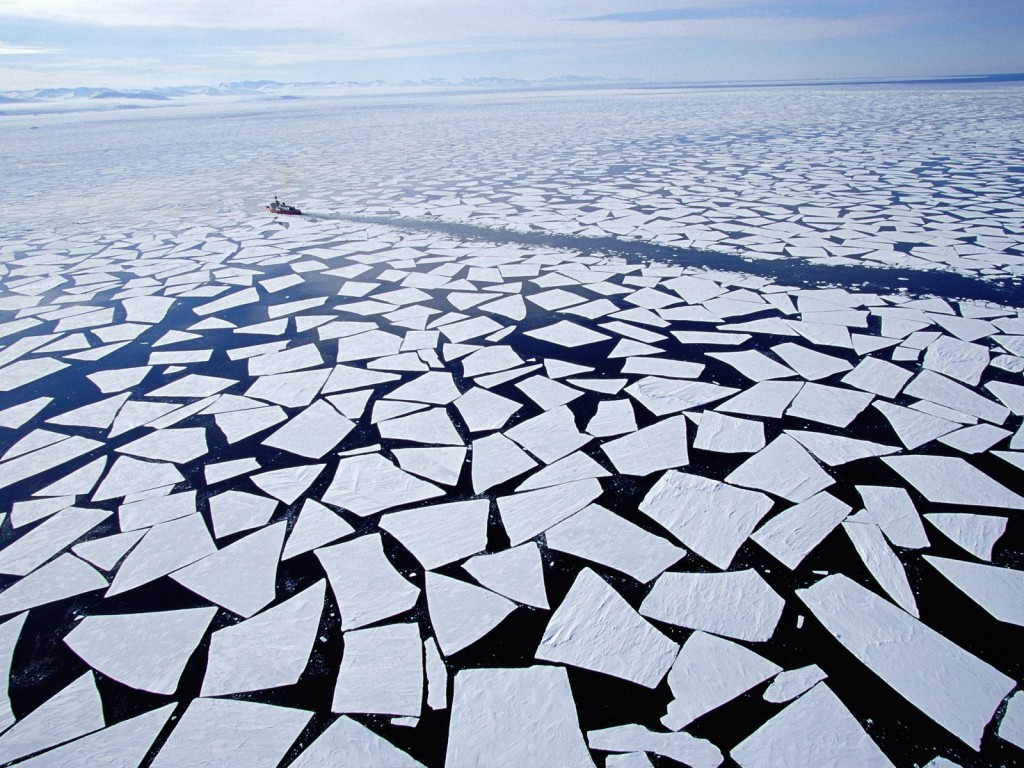
\includegraphics[width=0.5\linewidth]{images/icebreaker.jpg}
\end{figure}

\clearpage

\subsection*{Three Truths and a Lie}

Write down three truths and one lie about yourself on your piece of paper.  I'll guess which one is the lie!  
Good luck guessing which one is my lie.

\begin{itemize}
	\item I've seen over 100 different bands live in concert.
	\item I've programmed a human sized robot.  
	\item My family has 2 dogs.
	\item I've competed in and won a crib race.  
\end{itemize}

\clearpage

\subsection*{Concerts:  \color{ForestGreen} Truth}

\begin{figure}[h]
	\centering
\includegraphics[width=0.23\linewidth]{images/concert1.jpg}
\end{figure}

\clearpage

\subsection*{Robot:  \color{ForestGreen}  Truth}

\begin{figure}[h]
	\centering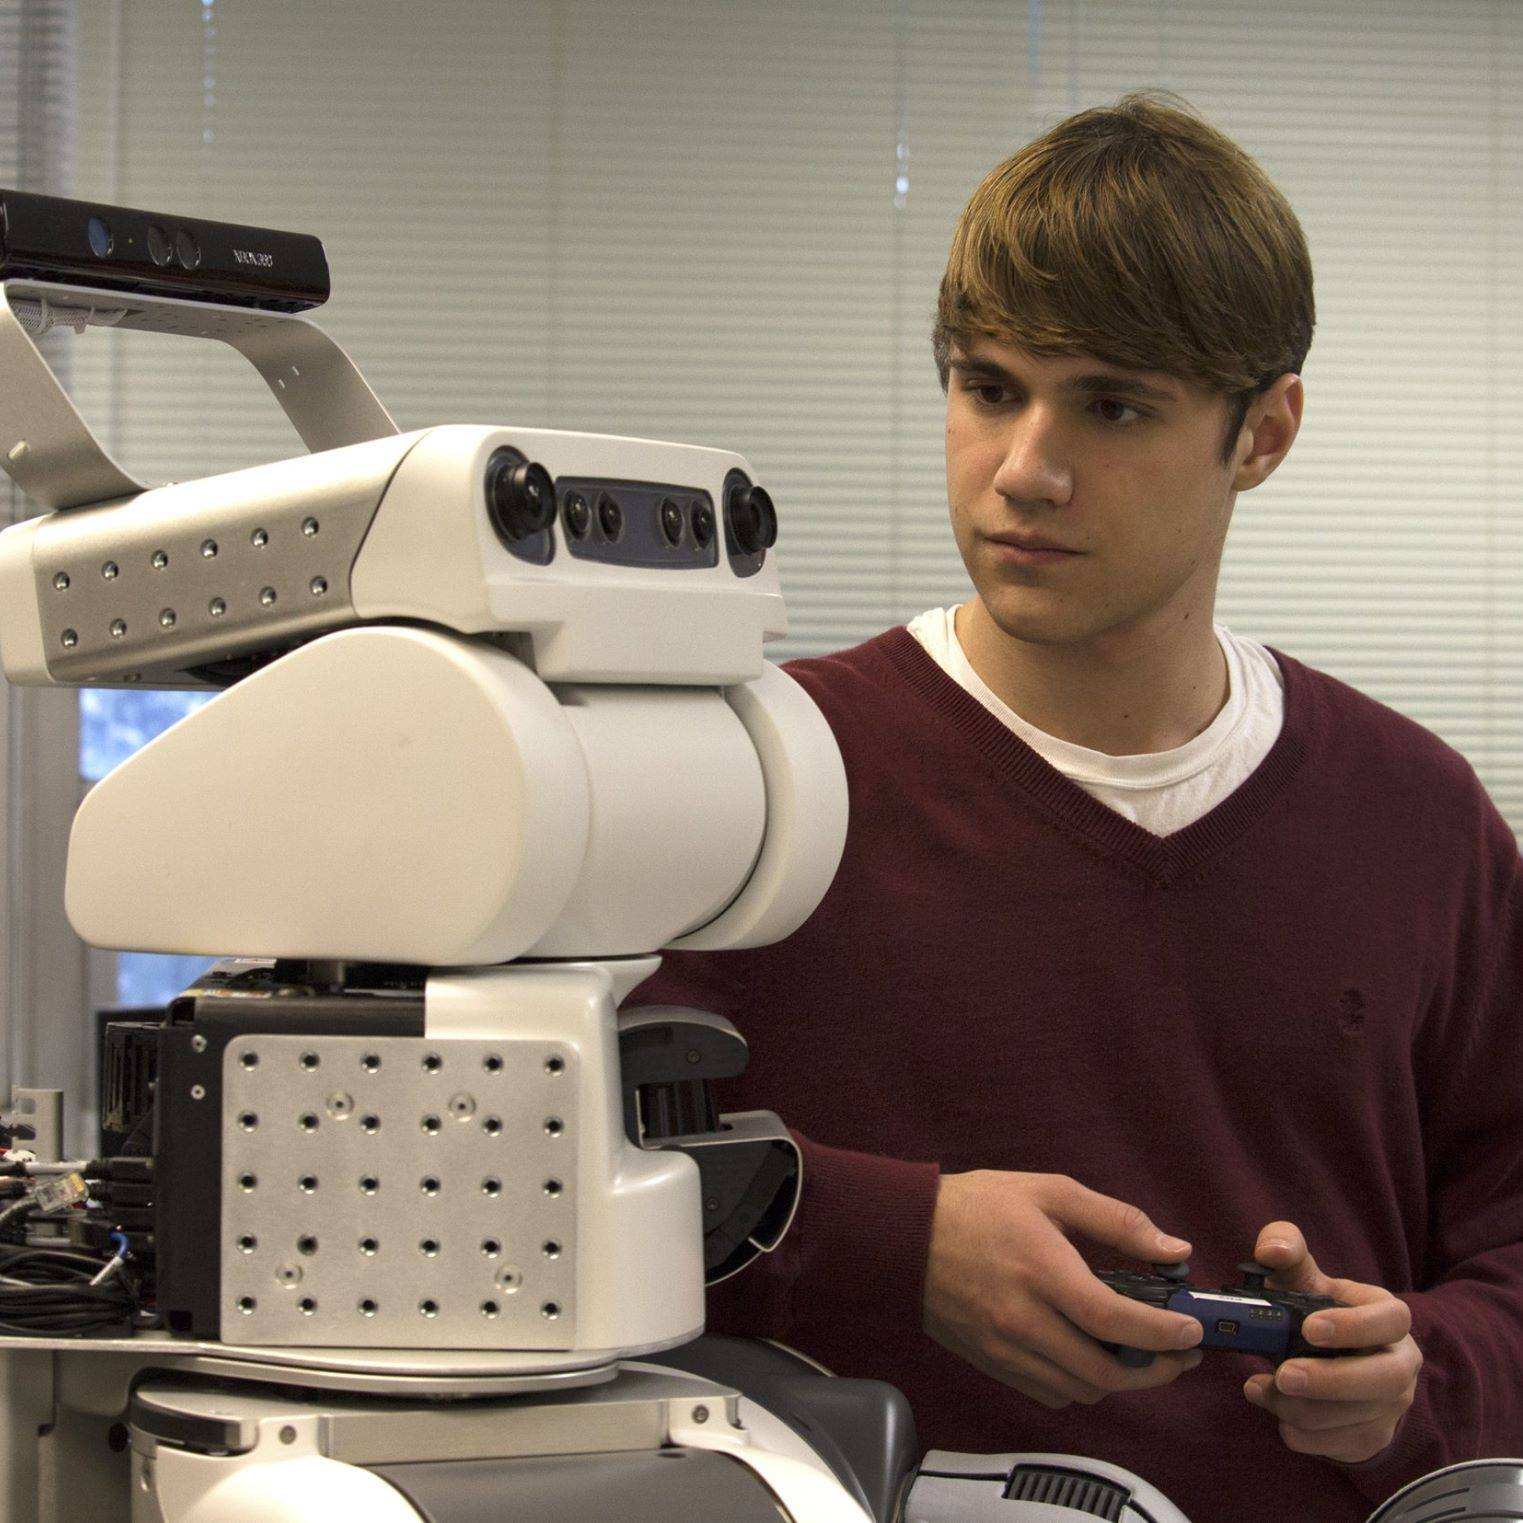
\includegraphics[width=0.4\linewidth]{images/robot.jpg}
\end{figure}

\clearpage

\subsection*{Dogs:  \color{red}  Lie!}

\begin{figure}[h]
	\centering
\includegraphics[width=0.4\linewidth]{images/lie.jpg}
\end{figure}

\clearpage

\subsection*{We have 5 cats though...}

\begin{figure}[h]
	\centering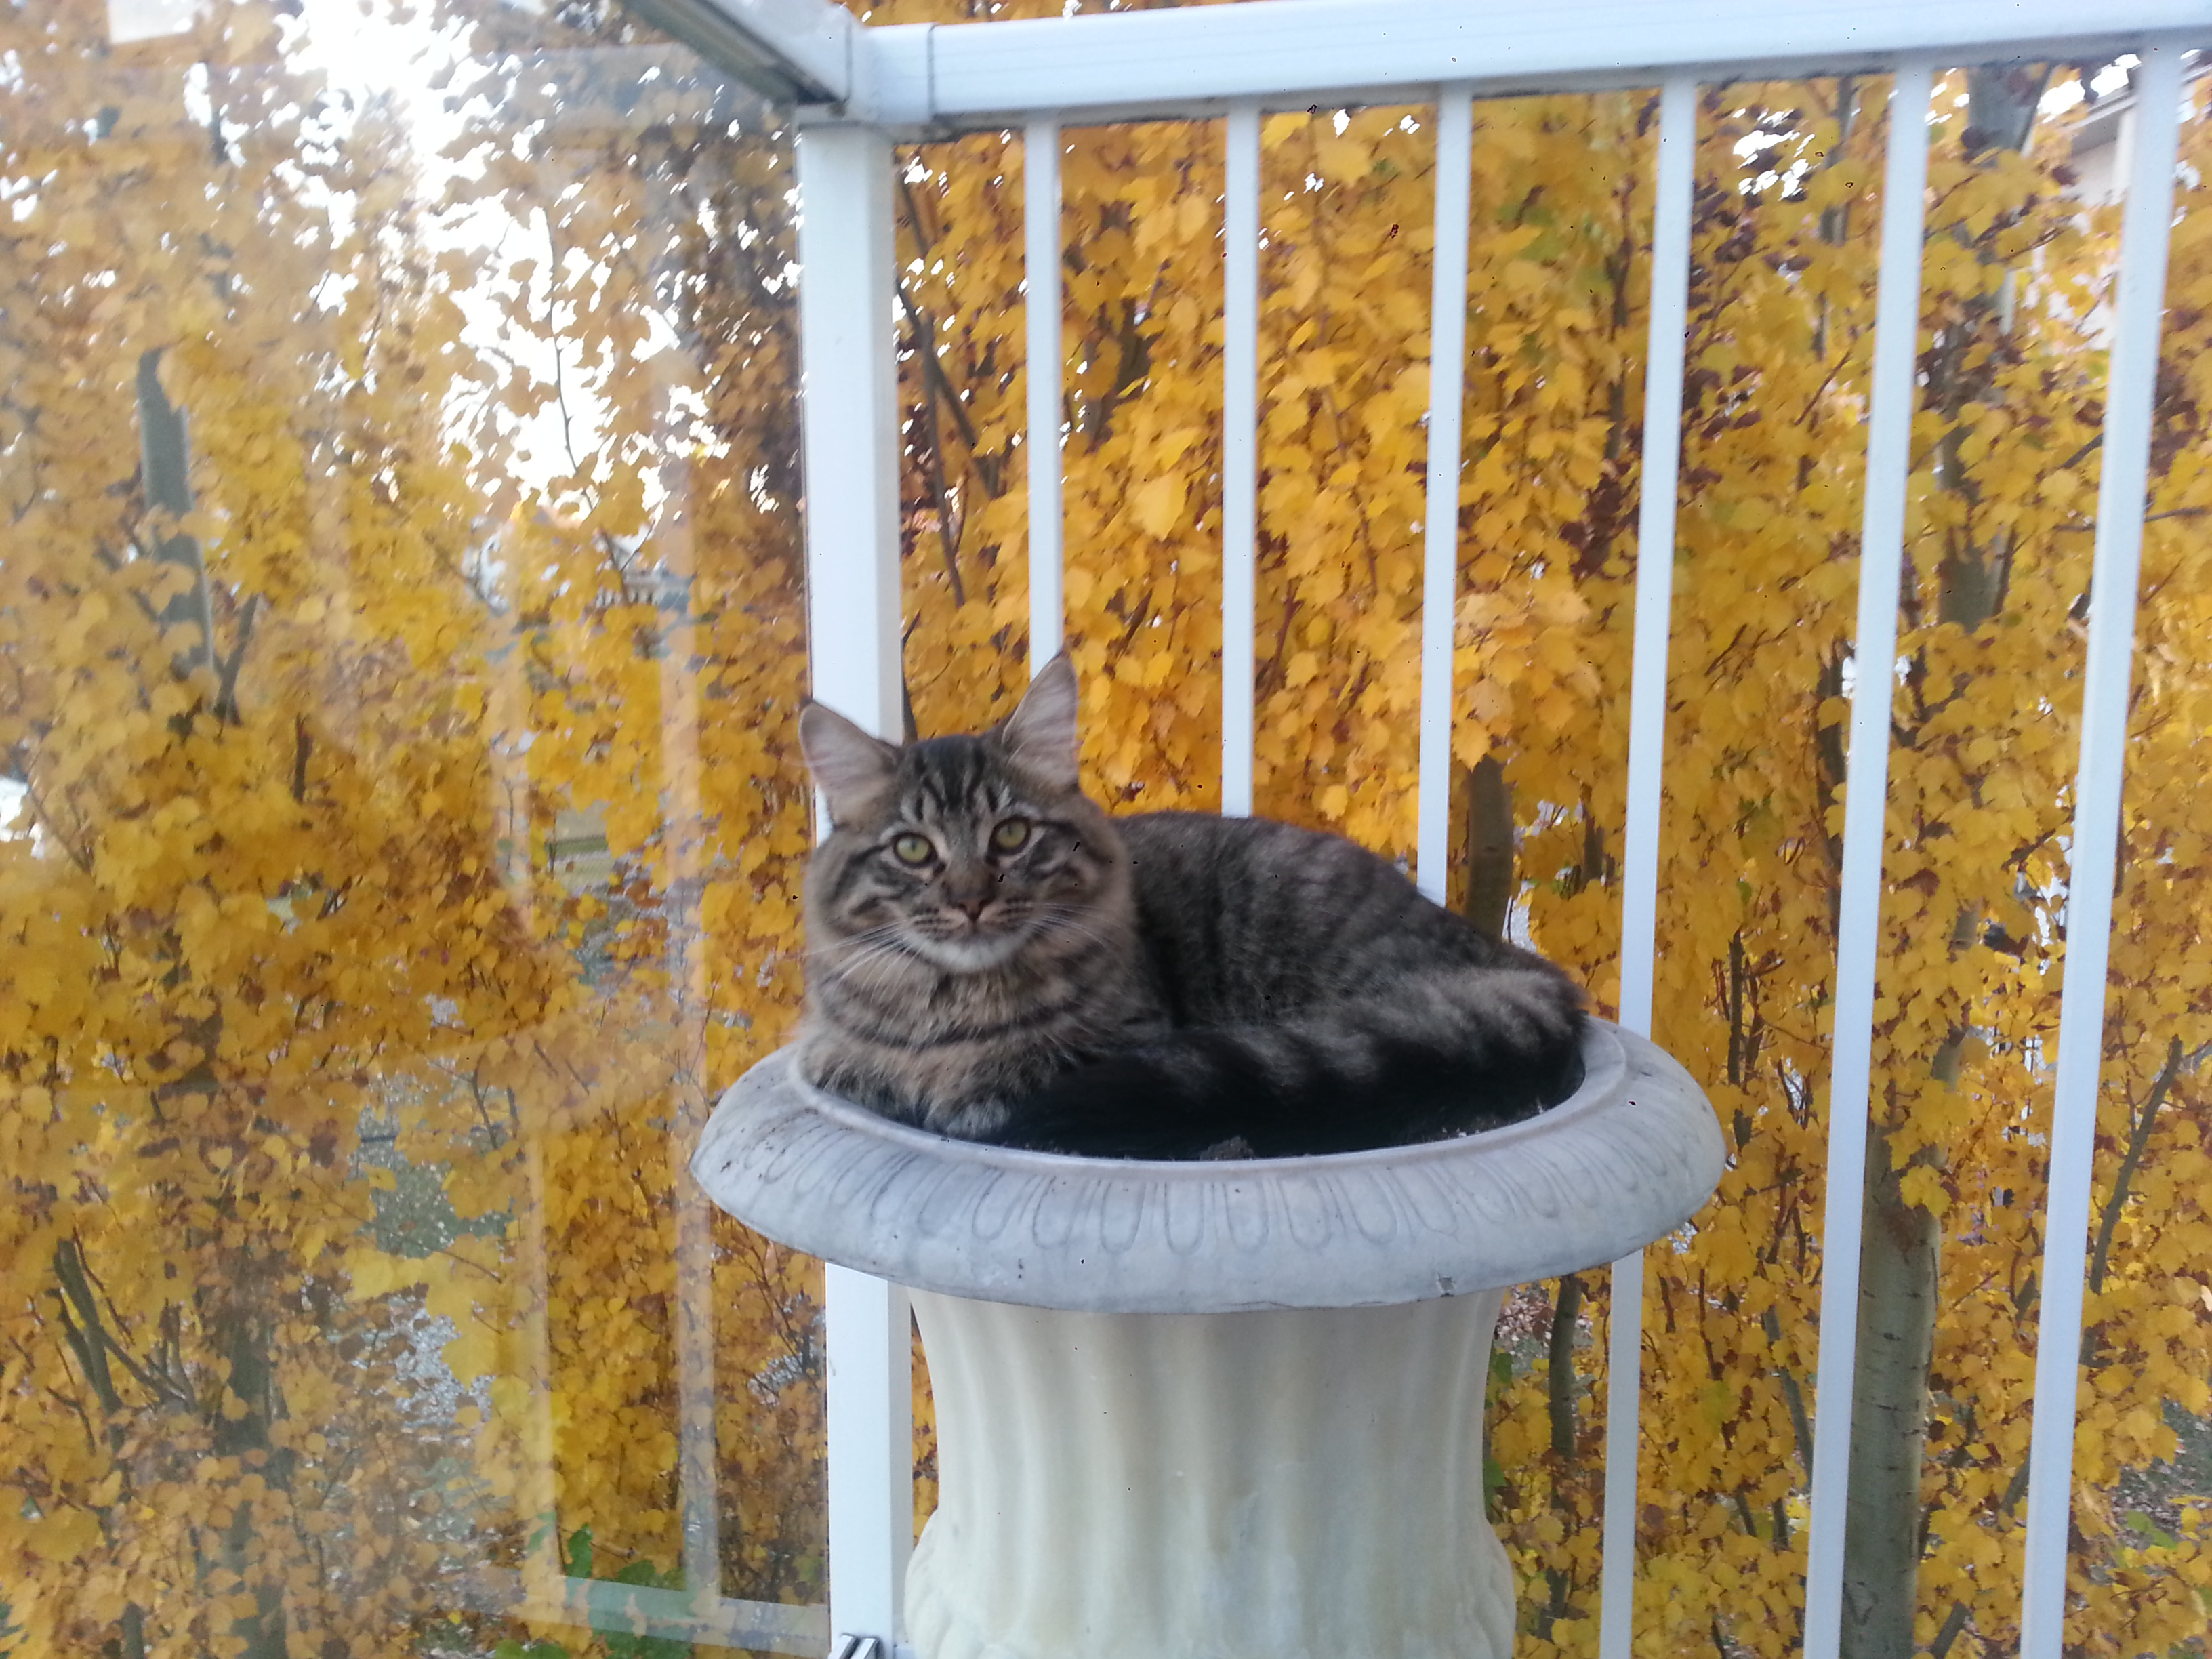
\includegraphics[width=0.5\linewidth]{images/creampuff.jpg}
\end{figure}

\clearpage

\begin{figure}[h]
	\centering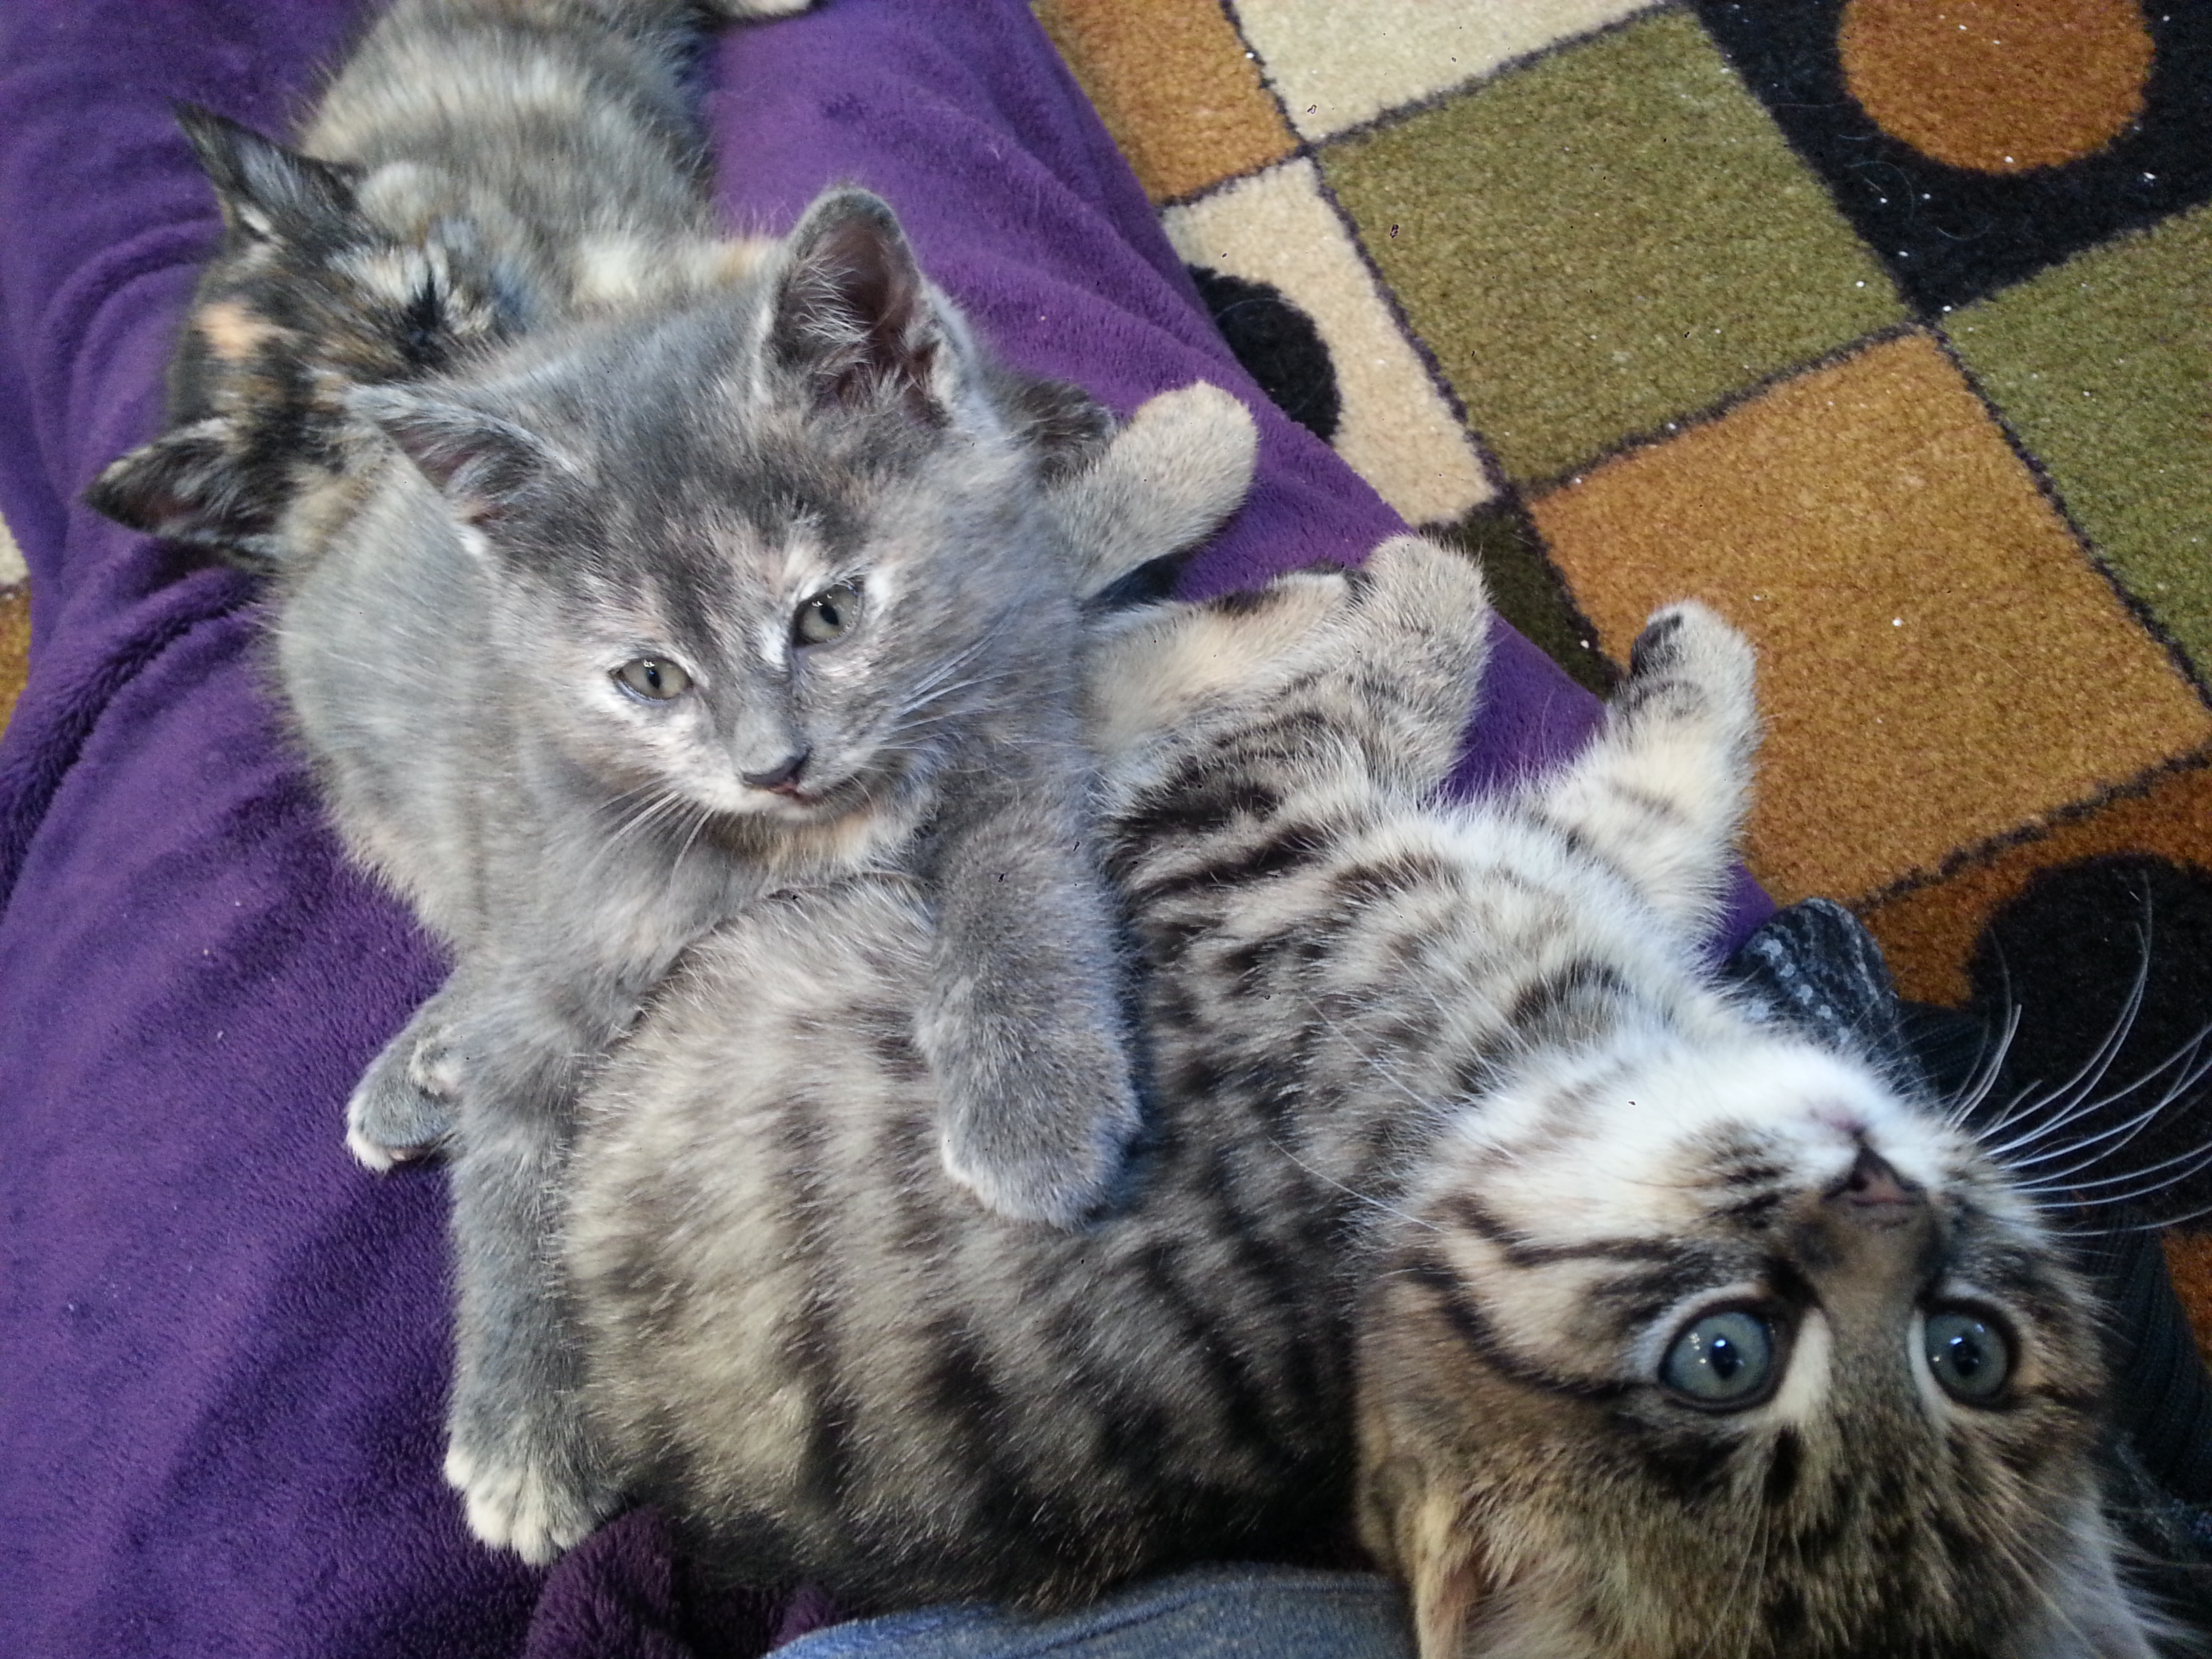
\includegraphics[width=0.6\linewidth]{images/kittens.jpg}
\end{figure}

\clearpage

%different picture of cupcake?
\begin{figure}[h]
	\centering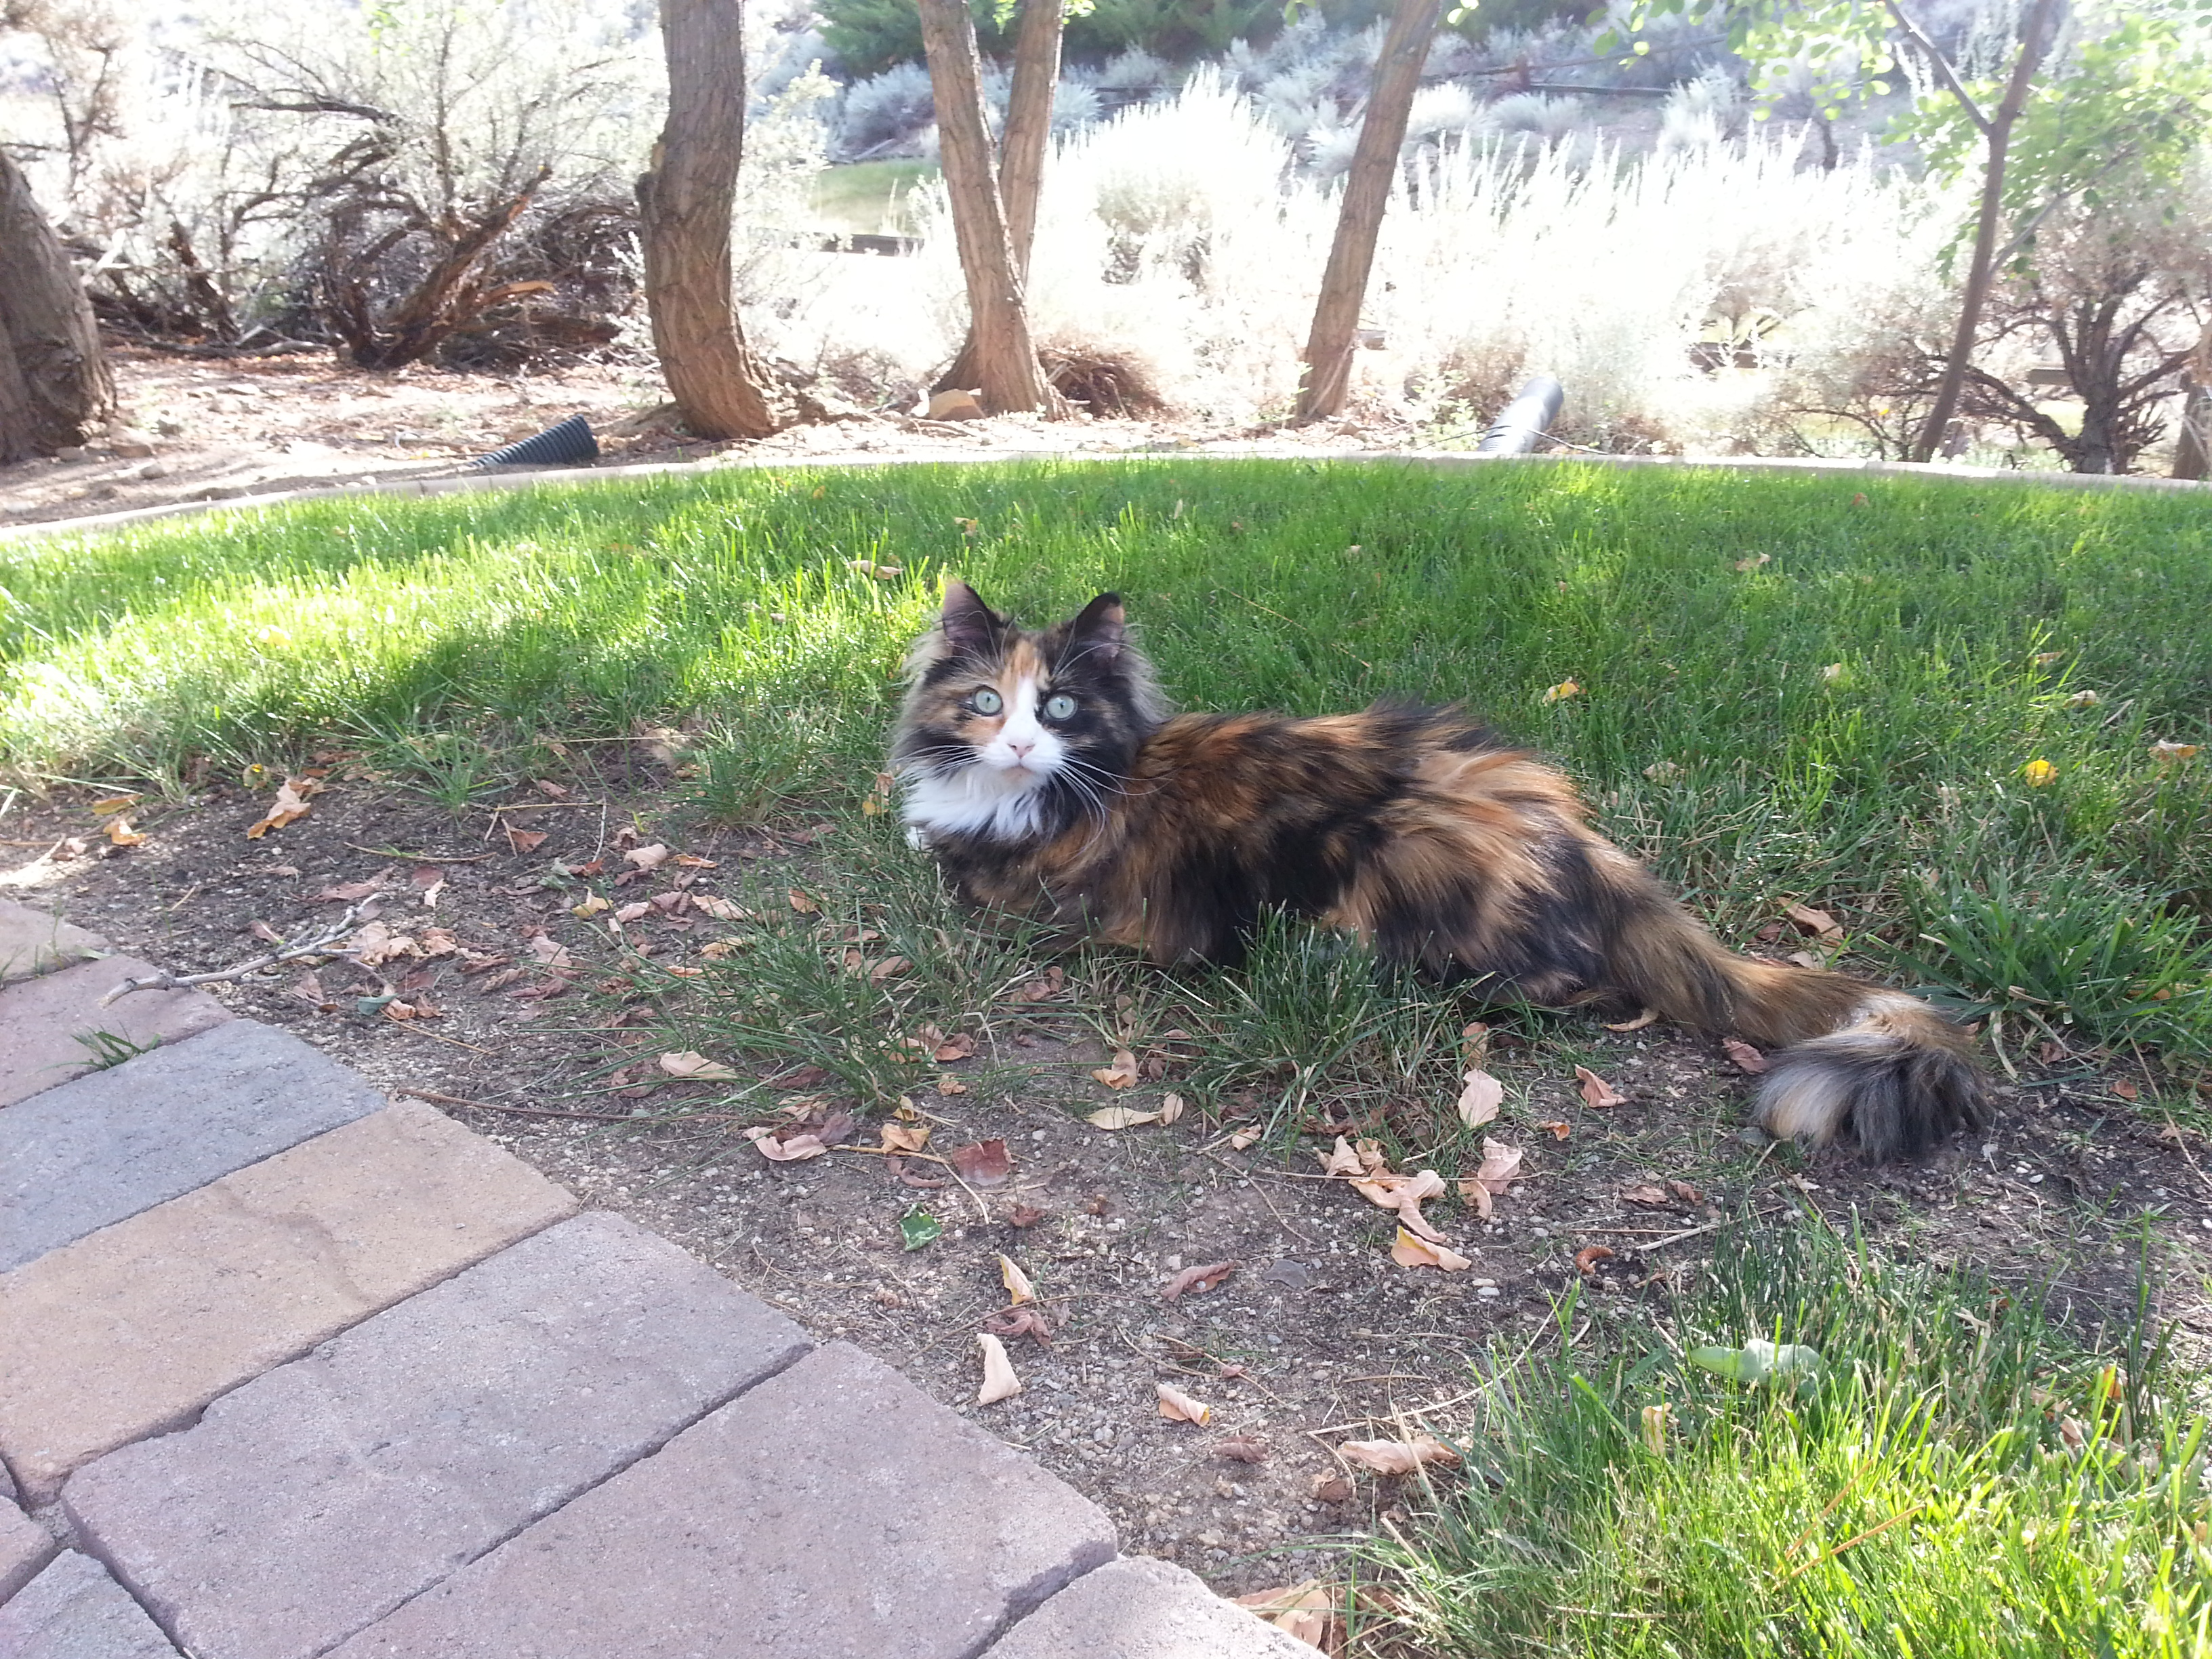
\includegraphics[width=0.6\linewidth]{images/cupcake.jpg}
\end{figure}

\clearpage 
\subsection*{Crib Race??:  \color{ForestGreen}  Truth}

\begin{figure}[h]
	\centering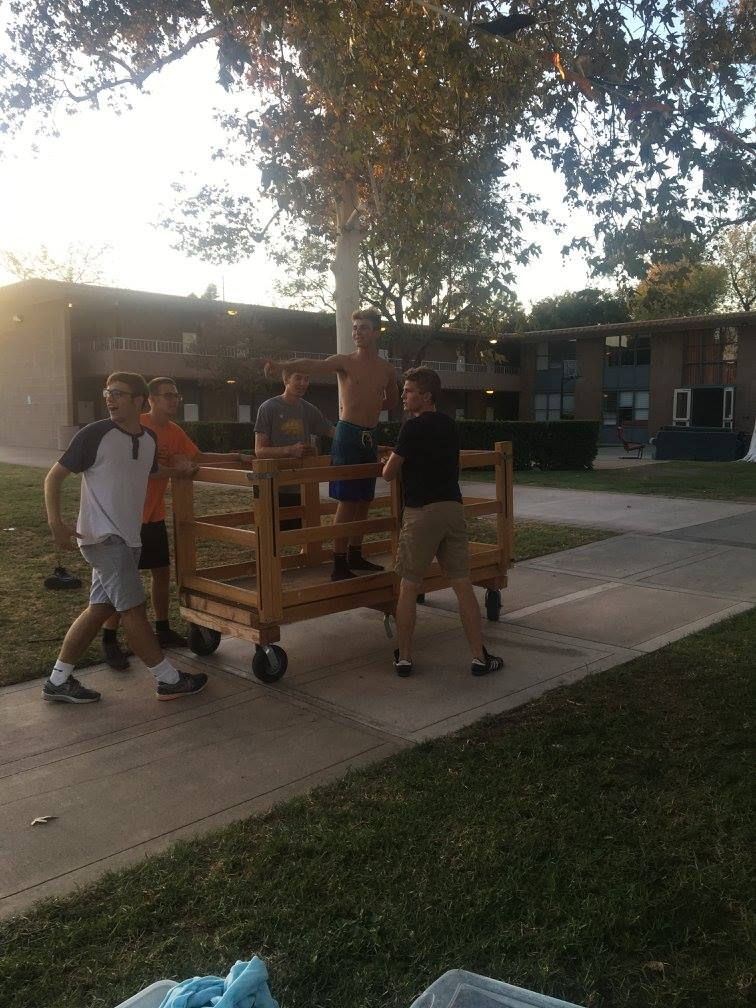
\includegraphics[width=0.32\linewidth]{images/crib.jpg}
\end{figure}

\clearpage
\subsection*{Celebration!}

\begin{figure}[h]
	\centering
\includegraphics[width=0.32\linewidth]{images/crib2.jpg}
\end{figure}

\clearpage  


%----------------------------------------------------------------------------------------
%	TABLE OF CONTENTS
%----------------------------------------------------------------------------------------

\thispagestyle{empty} % No slide header and footer

\small\tableofcontents % Change the font size and print the table of contents - it may be useful to shrink the font size further if the presentation is full of sections
% To exclude sections/subsections from the table of contents, put an asterisk after \(sub)section like so: \section*{Section Name}

\clearpage

\section{Divisibility Rules}

\begin{itemize}
\item  2 - Last digit is even. 
\item  3 - Sum of the digits is divisible by 3.
\item 4  - Number formed by last two digits is divisible by 4.
\item 5 - Last digit is either $0$ or $5$.
\item 6 -  Divisibility rules for both $2$ and $3$ hold.
\item 7  - Take the last digit of the number and double it.  Subtract this from the rest of the number.  Repeat the process if necessary.  Check to see if the final number obtained is divisible by $7$. \cite{a:1} 
\end{itemize}




\clearpage

\subsection*{Lucky Seven}

\begin{defi} When $a$ divides $b$, we write $a\mid b$. Another way of saying this is that $b$ is a multiple of $a$. \end{defi}

Choose \textbf{one} number below and determine if it is divisible by $7$.
\begin{itemize}
	\item $1729$
	\item $2,718,281$
	\item $16,180,339$
	\item $31,415,926,535$
\end{itemize}

\subsection*{Taxicab Number}

``It is a very interesting number; it is the smallest number expressible as the sum of two positive cubes in two different ways." -  Srinivasa Ramanujan (1919)
\begin{eqnarray*}
	1729 &\to& 172-2\cdot 9=154 \\ 
	154 &\to& 15-2\cdot 4=7
\end{eqnarray*}
Therefore, $1729$ \textbf{is} divisible by $7$.

Can you find the two ways Ramanujan referenced?  

\clearpage

\subsection*{Euler's Number}

\begin{eqnarray*}  
	2718281 &\to& 271828-2\cdot 1=271826 \\ 
	271826 &\to& 27182-2\cdot 6=27170 \\
	27170 &\to& 2717-2\cdot 0=2717 \\ 2717 &\to& 271-2\cdot 7=257 \\ 257 &\to& 25-2\cdot 7=11
\end{eqnarray*}

Therefore, $2718281$ is \textbf{not} divisible by $7$.

More on Euler's number ($e$) during Algebra lectures!  

\clearpage

\subsection*{The Golden Ratio - $\phi=\frac{1+\sqrt{5}}{2}=1.6180339\cdots$}

\begin{eqnarray*}
	16180339 &\to& 1618033-2\cdot 9=1618015 \\ 1618015 &\to& 161801-2\cdot 5=161791 \\ 161791 &\to& 16179-2\cdot 1=16177 \\ 16177 &\to& 1617-2\cdot 7=1603 \\ 1603 &\to& 160-2\cdot 3=154 \\ 154 &\to& 15-2\cdot 4=7
\end{eqnarray*}  

Hence, $16180339$ \textbf{is} divisible by $7$.

\clearpage

\subsection{Pi-ython Program}

$31,415,926,535$ is too big of a number.  Therefore, I wrote a computer program!

\begin{center} \Huge \href{https://github.com/musichead42/Teaching/blob/master/astar2016wmc/programs/Seven.ipynb}{Seven.ipynb} \end{center}
\normalsize

It \textbf{is} divisible by $7$.

\clearpage

\begin{figure}[h]
	\centering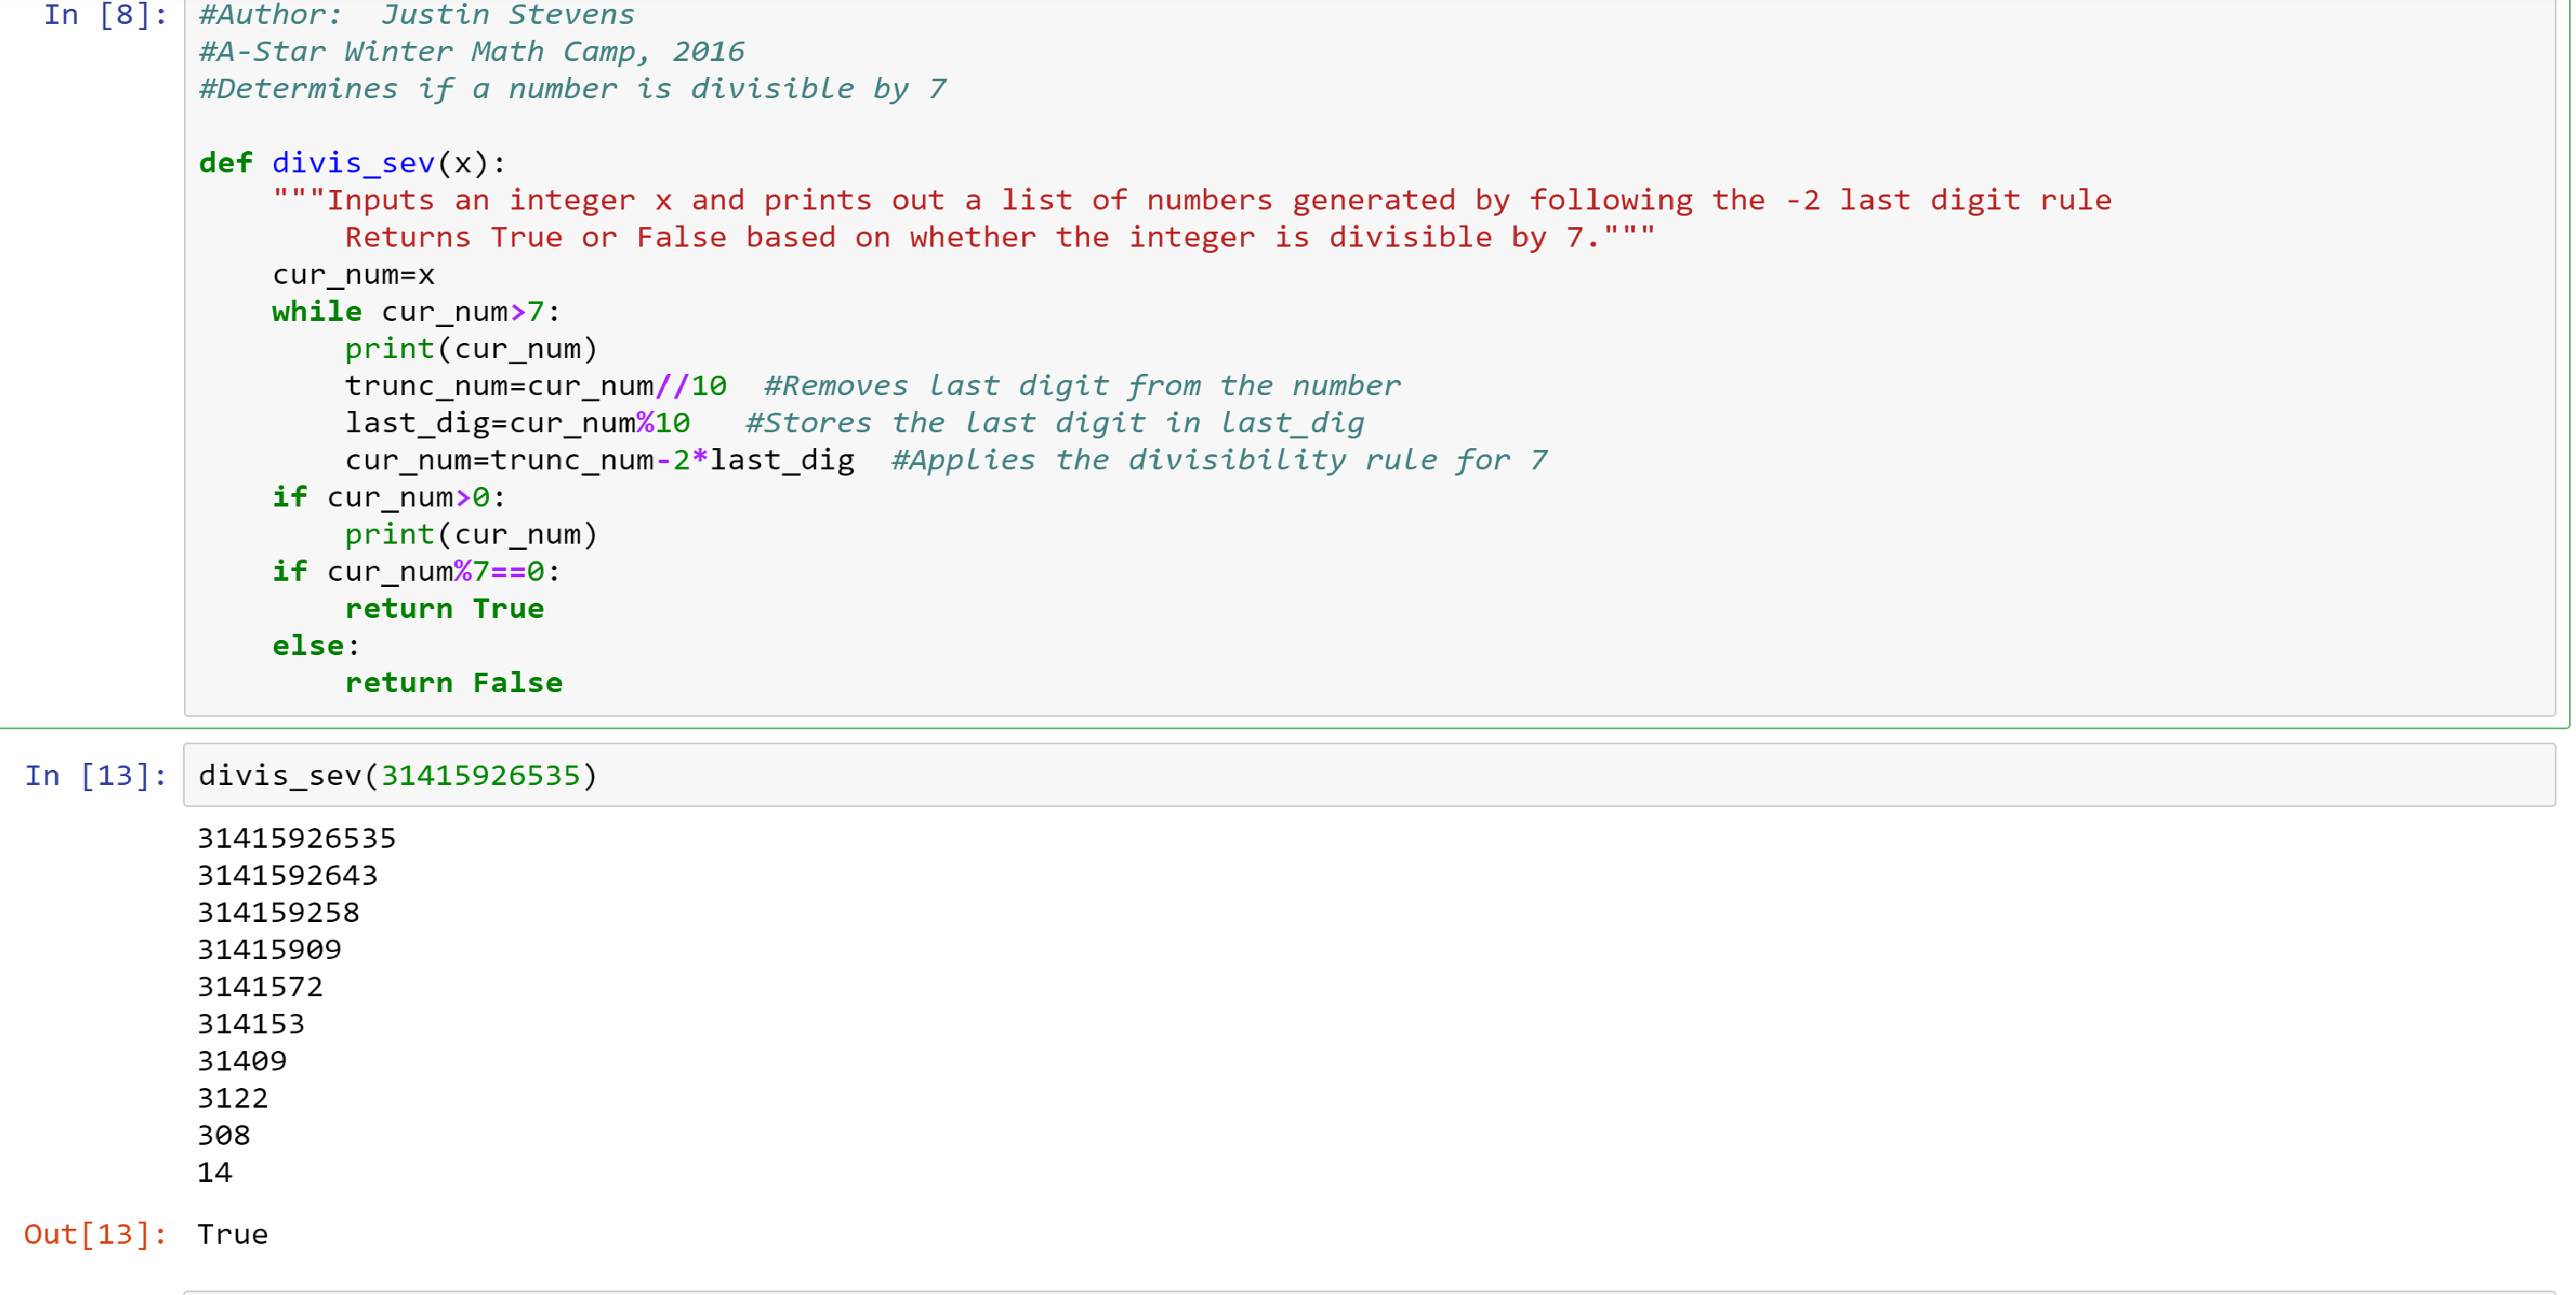
\includegraphics[width=1\linewidth]{images/seven.png}
\end{figure}
\clearpage

\subsection{Explanation of the Magic}

Let the number that we want to determine its divisibility by $7$ be $N$.  Let the last digit of $N$ be $x$.  Then, we can represent $N$ as $$N=10a+x.$$  

Note that we want to prove that $7$ divides $N$ implies that $7$ also divides $a-2x$.  

To do so, we will multiply $N$ by some integer.
\clearpage
\subsection*{Magic Continued}

The magic integer is $5$. The reason is because $5$ and $-2$ leave the same remainder when dividing by $7$.

If $7$ divides $N$, then $7$ should also divide $5N$.  From the expression above for $N$, we have $$5N=50a+5x.$$  Now, the question is, how do we get $a-2x$ out of this?  

\subsection*{Moving Around}

We think to take the difference between $5N$ and $a-2x$.  Since we know that $5N$ is divisible by $7$ if the difference is divisible by $7$, then $a-2x$ must also be divisible by $7$.

Using the expression for $5N$ we found on the previous slide, \begin{eqnarray*} 5N-(a-2x) &=& 50a+5x-(a-2x) \\ &=& 49a+7x. \end{eqnarray*}

This is clearly a multiple of $7$, therefore, our proof is complete!  





\clearpage

\subsection{More Divisibility Rules}

\begin{itemize}
	\item  8 - The numbers formed by the last three digits are divisible by $8$.
	\item 9 - The sum of the digits is divisible by $9$.
	\item 10 - The number ends in $0$.
	\item 11 - Let $E$ be the sum of the digits in an even place. Let $O$ be the sum of the digits in an odd place. $11$ must divide the difference $E-O$ for the number to be divisible by $11$.
	\item 12 - Combination of divisibility rules for $3$ and $4$.
	\item 13 -  Same as the divisibility rule for $7$, except replace $-2x$ with $+4x$.  
\end{itemize}

\subsection{Eleven}

Let $N=1734579.$ We check to see if $N$ is divisible by $11$. We begin labeling the digits beginning by labeling $9$ as $0$. Why $0$? Think of how lists are stored in Python! Then $7$ is labeled as $1$, $5$ is labeled as $2$, and so forth. We make all of the \color{red} even \color{black} digits red and all of the \color{blue} odd \color{black} digits blue.
$$N=\color{red}1\color{blue}7\color{red}3\color{blue}4\color{red}5\color{blue}7\color{red}9.$$ Then, we calculate the sum of the even digits and odd digits: $$\color{red} E=1+3+5+9=18\:, \color{blue}O=7+4+7=18.$$ Note that $E-O=18-18=0$, which is divisible by $11$, therefore, $11$ divides $N$.  

\section{Factorials}

One of my favourite problems in number theory has to do with factorials. The factorial of a positive integer $n$ is defined as the product of all the natural numbers less than or equal to $n$. In other words, $$n!=n\times (n-1)\times (n-2)\times \cdots 1.$$  For instance, $6!=6\times 5\times 4\times 3\times 2\times 1=720$.

\subsection{Zeros at the end of a Factorial}

Note that $6!=720$ ends in one zero.  The number $$25!=15511210043330985984000000$$ ends in $6$ zeros. 

\mybox{0.8\textwidth}{\begin{prob} How many zeros does $100!$ end in?  \end{prob}}
\clearpage 

\subsection*{How Does Zero Work?}

Zeros at the end of a number come from powers of $10$.  For instance, we can rewrite $$25!=15511210043330985984\times 10^6.$$  
Therefore, the problem is equivalent to finding the largest power of $10$ that divides $100!$.  \begin{defi}  Define $v_p(n)$ to be the integer $e$ such that $p^e\mid n$, but $p^{e+1}\nmid n$. Another way to write this is $p^e\pmid n$. \end{defi} 

\clearpage



\subsection{V for Vendetta}

We desire to find $v_{10}(100!)$.  Since $10=2\cdot 5$, the largest power of $10$ that divides $100!$ is the \textbf{minimum} of $v_2(100!)$ and $v_5(100!)$.   

We begin by calculating $v_2(100!)$. We write out $$100!=100\cdot 99\cdot 98\cdot 97\cdots 3\cdot 2\cdot 1.$$  Consider all the numbers in the product above. 

How many of them are multiples of 2?  Multiples of 4?  Multiples of 8?  Multiples of 16?  Multiples of 32?  Multiples of 64?  

\clearpage 

\subsection*{Floor Function}

The number of multiples of $2$ in $100!$ is simply the number of even numbers in the product. Half of the numbers are even, therefore, there are $\frac{100}{2}=50$ multiples of $2$.  

For other powers of $2$ that do not evenly divide into $100$, we must introduce the floor function.  

\begin{defi} The floor function of a real number $x$ is defined as the largest integer less than or equal to $x$. In other words, it is the result of truncating $x$. For instance, $\lfloor 3.14159 \rfloor=3$ and $\lfloor -16.3 \rfloor=-17$. \end{defi}

\clearpage

Using our new friend, the floor function, we answer the question about multiples.
\begin{itemize}  
	\item  There are $\lfloor \frac{100}{2} \rfloor=50$ multiples of $2$.
	\item  There are $\lfloor \frac{100}{4} \rfloor=25$ multiples of $4$.
	\item  There are $\lfloor \frac{100}{8} \rfloor=12$ multiples of $8$.
	\item  There are $\lfloor \frac{100}{16} \rfloor=6$ multiples of $16$.
	\item  There are $\lfloor \frac{100}{32} \rfloor=3$ multiples of $32$.
	\item  There are $\lfloor \frac{100}{64} \rfloor=1$ multiple of $64$.  
\end{itemize}

\subsection*{How Much Power Does 2 Have?}

I claim that the number of powers of $2$ in $100!$ is the sum of all the numbers above: $$50+25+12+6+3+1=97.$$  

For the numbers in the product $100!$ that have a highest power of $2^{1}$, we have counted them once in the number $50$. 

For those that have a highest power of $2^{2}$, they contribute a total of $2$ to the product $100!$. We have counted them \textit{once already} in the number $50$ since they are also multiples of $2$. Since they should contribute a total of $2$ to the product, we add them one time more in the number $25$.  
\clearpage

Similarly, for the numbers that have a highest power of $2^3$, they should contribute a total of $3$ to the product $100!$. They have been counted once in the number $50$ and once in the number $25$, therefore, we should add them one time more in the number $12$.

This logic extends to the powers $2^4, 2^5$, and $2^6$.  

Hence, $v_2(100!)=97$.  Are we done now?

\clearpage

\subsection*{Forgot About Magic 5}

Nope! We also must compute $v_5(100!)$. We use the same method as above to determine that:
\begin{itemize}
	\item There are $\lfloor \frac{100}{5} \rfloor=20$ multiples of $5^1$.
	\item There are $\lfloor \frac{100}{25} \rfloor=4$ multiples of $5^2$.
\end{itemize} 

Therefore, $v_5(100!)=20+4=24$.  

\clearpage

\subsection*{Finishing the Problem}

Therefore, $5^{24}\pmid 100!$ and $2^{97}\pmid 100!$.  Hence, the largest power of $10$ that divides $100!$ is $24$ and the number of zeros at the end of $100!$ is $\framebox{24}$.   

We indeed verify through the use of Mathematica that

$100!=\seqsplit{%9332621544394415268
				10699238856266700490715 96826438162146859296389
				52175999932299156089414
				6397615651828625369792082
				7223758251185210916864
				000000000000000000000000.}$

\clearpage

\subsection{Legendre's Formula}

Adrien-Marie Legendre (1752-1833) generalized this problem.  

\mybox{0.8\textwidth}{\begin{theorem} The number of powers of a prime $p$ that divide into $n!$ is $$v_p(n!)=\sum_{k=1}^{\infty}\left(\left\lfloor \frac{n}{p^k} \right\rfloor\right).$$   \end{theorem}}

\clearpage

\subsection*{Summation Symbol}

The $\sum$ symbol represents a summation. The $k$ at the bottom is the variable that is being summed over. The $1$ and $\infty$ are the ranges for the sum. For instance, $$\sum_{k=1}^{4}(k^2)=1^2+2^2+3^2+4^2.$$  
In the case of the sum above, $$\sum_{k=1}^{\infty}\left(\left\lfloor \frac{n}{p^k} \right\rfloor\right)=\lfloor \frac{n}{p^1}\rfloor+\lfloor \frac{n}{p^2}\rfloor+\lfloor \frac{n}{p^3} \rfloor+\lfloor \frac{n}{p^4} \rfloor+\cdots.$$  

\clearpage 

Define $s_p(n)$ to be the sum of the digits when the number $n$ is expressed in base $p$. Then, an alternative way of writing Legendre's Formula is $$v_p(n!)=\frac{n-s_p(n)}{p-1}.$$  

For instance, $100$ in base $2$ is $100=1100100_2$. The sum of the digits is $s_2(100)=3$. Therefore, $$v_2(100!)=\frac{100-3}{1}=97.$$ 
Furthermore, $100=400_5$. The sum of the digits is $s_5(100)=4$. Therefore, $$v_5(100!)=\frac{100-4}{4}=24.$$

\clearpage

\section{Euclid's Elements}

Around the time of 300 BC, a great Greek mathematician rose from Alexandria by the name of Euclid. He wrote a series of 13 books known as \textit{Elements}. Elements is thought by many to be the most successful and influential textbook ever written. It has been published the second most of any book, next to the Bible. \cite{wiki:el}

The book covers both Euclidean geometry and elementary number theory. This chapter will focus solely on \textbf{Book VII, Proposition 1.}

\clearpage

\begin{figure}[h]
	\centering\includegraphics[width=0.30\linewidth]{images/euclid.jpg}
	\caption{``Frontispiece of Sir Henry Billingsley's first English version of Elements in 1570" - Source:  Wikipedia \cite{wiki:el}}
\end{figure}

\clearpage

\subsection{Division Algorithm} 
The way division is commonly introduced in primary school is seen in the picture below:

\begin{figure}[h]
	\centering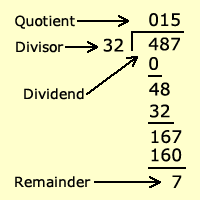
\includegraphics[width=0.25\linewidth]{images/divisionparts.png}
	\caption{Source:  CalculatorSoup}
\end{figure}

\clearpage

The division algorithm rigorizes this process. In the integers, $\mathbb{Z}$, the statement of the division algorithm is below:

\mybox{0.8\textwidth}{\begin{theorem} For every integer pair $a,b$, there exists distinct integer quotients and remainders, $q$ and $r$, that satisfy \begin{eqnarray*} a=bq+r &|& 0\le r<|b|. \end{eqnarray*} \end{theorem}}

The proof of this comes from either the well-ordering principle or induction. We show the proof involving the well-ordering principle.

\begin{proof}

We consider the case when $b$ is positive for simplicity.  Consider the set \begin{eqnarray*} S=\{a-bq &|& q \in \mathbb{Z}^{+},\:a-bq>0\}. \end{eqnarray*}  
In other words, this set consists of the positive integer values of $a-bq$ for $q$ also being a positive integer.  In order to continue with the proof, we must cite a famous Lemma from set theory.  \cite{me:1} 

\mybox{0.8\textwidth}{\begin{lemma}[Well-ordering principle]  Every non-empty subset of positive integers has a least element.  \end{lemma}} 

\clearpage

Therefore, the set $S$ has a \textit{minimum element}, say when $q=q_1$ and $r=r_1$. I will prove that $0\le r_1<b.$  

Assume for the sake of contradiction otherwise and that \begin{eqnarray} a-bq_1=r_1\ge b. \label{eqn: div} \end{eqnarray} However, then I claim that $a-b(q_1+1)$ is a smaller member of set $S$. 

Indeed, since $q_1+1\in \mathbb{Z}^{+}$, the first condition is satisfied.

Furthermore, using \ref{eqn: div}, $a-b(q_1+1)=a-bq_1-b\ge 0$. Therefore, both conditions are satisfied, and we have found a smaller member of set $S$. This contradicts the minimality of $q_1$ and $r_1$.  Hence, $0\le r_1<b$.   \end{proof}

\clearpage

\subsection*{Examples of Division Algorithm}

When $a=102$ and $b=18$, applying the division algorithm gives $$102=18\times 5+12,$$ therefore $q=5$ and $r=12$. 

\mybox{0.8\textwidth}{\begin{exmp}  Find $q$ and $r$ when $a=2016$ and $b=37$.  \end{exmp}}
\clearpage


\begin{defi}  We define the \textbf{greatest common divisor} of two integers to be the largest positive integer that divides both of the numbers. We define the \textbf{least common multiple} of two integers to be the smallest positive integer that is a multiple of both numbers.  \end{defi}

Note that in the previous example, $\gcd(a,b)=\gcd(102, 18)=6$. Similarly, $\gcd(b, r)=\gcd(18, 12)=6$. 

In the other example, we have $2016=37\cdot 54+18$. Hence, $q=54$ and $r=18$. Furthermore, $\gcd(a,b)=\gcd(2016, 37)=1$ and $\gcd(b,r)=\gcd(37, 18)=1$. 

Therefore, we conjecture that in general, $\gcd(a,b)=\gcd(b,r).$ 
\clearpage

\subsection{Book VII, Proposition 1}

\begin{displayquote} ``When two unequal numbers are set out, and the less is continually subtracted in turn from the greater, if the number which is left never measures the one before it until a unit is left, then the original numbers are relatively prime." - Euclid \end{displayquote}

\mybox{0.8\textwidth}{\begin{theorem}  Given naturals $a,b$, upon using the division algorithm to obtain a quotient and remainder, $q,r$, one has that $\gcd(a,b)=\gcd(b,r)$. \end{theorem}}

\clearpage

\begin{proof}

I claim that the set of common divisors between $a$ and $b$ is the same as the set of common divisors between $b$ and $r$.  

If $d$ is a common divisor of $a$ and $b$, then since $d$ divides both $a$ and $b$, $d$ divides all linear combinatinations of $a$ and $b$.  Therefore, $d\mid a-bq=r$, meaning that $d$ is also a common divisor of $b$ and $r$.  

Conversely, if $d$ is a common divisor of $b$ and $r$, then $d$ is a common divisor of all linear combinations of $b$ and $r$, therefore, $d\mid bq+r=a$.  Hence, $d$ is also a common divisor of $a$ and $b$.  

We have established that the two sets of common divisors are equivalent, therefore, the greatest common divisor must be equivalent.  \end{proof}

\clearpage

\begin{theorem}[Euclidean Algorithm]  For two natural $a,b$, $a>b$, to find $\gcd(a,b)$ we use the division algorithm repeatedly  \begin{eqnarray*}  a&=&bq_1+r_1 \\ b&=&r_1q_2+r_2 \\ r_1&=&r_2q_3+r_3 \\ \cdots \\ r_{n-2}&=&r_{n-1}q_n+r_n \\ r_{n-1}&=&r_nq_{n+1}. \end{eqnarray*}  
	Then we have $\gcd(a, b)=\gcd(b, r_1)=\cdots=\gcd(r_{n-1}, r_n)=r_n.$  \end{theorem}
\clearpage

\subsection*{Examples of Euclidean Algorithm}

Note that the greatest common divisor is the \textit{last non-zero remainder}. 
\begin{itemize}
		\item Find $\gcd(301, 603)$.  
		\item  Find $\gcd(110, 490)$.
		\item  Find $\gcd(153, 289)$.
		\item  Find $\gcd(481, 2627)$. 
\end{itemize}
\begin{itemize}[label=$\star$]
		\item Find $\gcd(1558, 8774)$. 
\end{itemize} 

We'll discuss our findings in a few minutes!

\clearpage

\mybox{0.8\textwidth}{\begin{prob} Find $\gcd(301, 603)$. \end{prob}}

\begin{proof}[Solution]  
Note that $$603=301\times 2+1.$$  Therefore, by the Euclidean Algorithm, we have $$\gcd(603, 301)=\gcd(1, 301)=\framebox{1}.$$ 

\end{proof}

\clearpage

\mybox{0.8\textwidth}{\begin{prob}  Find $\gcd(110, 490)$.  \end{prob}}

\begin{proof}[Solution]
	 We repeatedly use the division algorithm as follows: 
	 \begin{eqnarray*} 490&=&110\times 4+50 \\ 110&=&50\times 2+\framebox{10} \\ 50&=&10\times 5.\end{eqnarray*} 
Therefore $\gcd(110, 490)=\framebox{10}$.  \end{proof} 

\clearpage

\mybox{0.8\textwidth}{\begin{prob}  Find $\gcd(153, 289)$.  \end{prob}}

\begin{proof}[Solution]
	We repeatedly use the division algorithm as follows:
		\begin{eqnarray*}  289 &=& 153\times 1+136 \\ 153 &=& 136\times 1+\framebox{17} \\ 136&=& 17\times 8+0. \end{eqnarray*}
Therefore $\gcd(153, 289)=\framebox{17}$.  \end{proof}

\clearpage

\mybox{0.8\textwidth}{\begin{prob} Find $\gcd(481, 2627)$. \end{prob}}

\begin{proof}[Solution]
We repeatedly use the division algorithm as follows: 
	\begin{eqnarray*}  
	2627 &=& 481\times 5+222 \\
	481 &=& 222\times 2+\framebox{37} \\
	222 &=& 37\times 6+0 
	\end{eqnarray*}
Therefore $\gcd(481, 2627)=\framebox{37}$. 
\end{proof}

\clearpage

\subsection{Mathematica Function: QuotientRemainder}

\mybox{0.8\textwidth}{\begin{prob} 	Find $\gcd(1558, 8774)$. \end{prob}}

\begin{proof}[Solution]
	
I'm going to use Mathematica to assist me. On Mathematica, I can compute the quotient and remainder with the command \begin{center} QuotientRemainder(8774, 1558). \end{center}

The output of this command is \{5, 984\}. Here, $q=5$ and $r=984$.  

Therefore, $8774=1558\times 5+984.$

\clearpage

From this image, can you determine what $\gcd(1558, 8774)$ is? \end{proof}

\begin{figure}[H]
	\centering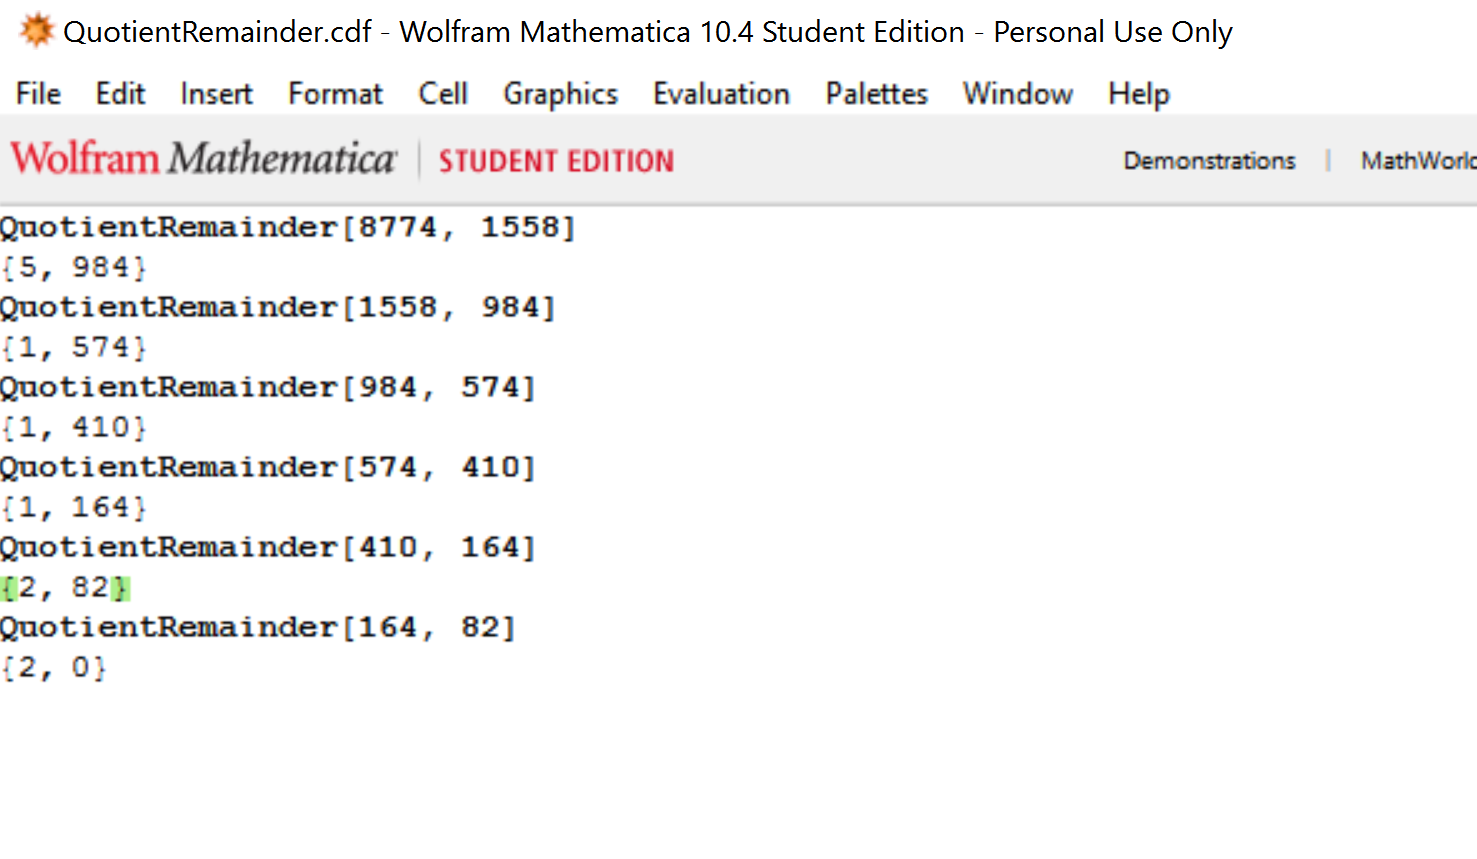
\includegraphics[width=0.8\linewidth]{images/quotient.png}
\end{figure}

\clearpage

\section{Contest Style Euclidean Algorithm Problems}
\mybox{0.9\textwidth}{\begin{prob}[AIME 1986] What is the largest positive integer $n$ such that $n^3+100$ is divisible by $n+10$? \end{prob} \begin{prob}[AIME 1985]  The numbers in the sequence $101, 104, 109, 116, \dots$ are of the form $a_n = 100 + n^2$, where $n = 1, 2, 3, \dots$.  For each $n$, let $d_n$ be the greatest common divisor of $a_n$ and $a_{n + 1}$.  Find the maximum value of $d_n$ as $n$ ranges through the positive integers.  \end{prob}}

\subsection{AIME 1986 \#5}

\begin{proof}[Solution] We desire to find out when $n+10$ divides $n^3+100$. To get a good sense for the problem, we attempt to divide $n^3+100$ by $n+10$ using unknown coefficients: \begin{eqnarray*}  n^3+100&=&\left(n+10\right)\left(n^2+an+b\right)+c \\ &=&n^3+n^2\left(10+a\right)+n\left(b+10a\right)+10b+c. \end{eqnarray*}

Next, we must equate coefficients on the two sides in order to find the quotient and remainder. 
\clearpage 
Equating coefficients yields 
\begin{eqnarray*}
		10+a&=&0 \\ 
		b+10a&=&0 \\ 
		10b+c&=&100. \end{eqnarray*} Solving this system of equations gives $a=-10, b=100, c=-900$.  
Therefore, $$n^3+100=(n+10)(n^2-10n+100)-900.$$

\clearpage

If $n+10$ divides $n^3+100$, then we must have $\gcd(n^3+100, n+10)=n+10$. By the Euclidean Algorithm, $\gcd(n^3+100, n+10)=\gcd(900, n+10)$. Therefore, equating the two, we must have $$\gcd(900, n+10)=n+10.$$ Hence, the largest possible value of $n$ is when $n=\framebox{890}$. \end{proof}  

\clearpage

\subsection{AIME 1985 \#13}

\begin{prob} The numbers in the sequence $101, 104, 109, 116, \dots$ are of the form $a_n = 100 + n^2$, where $n = 1, 2, 3, \dots$.  For each $n$, let $d_n$ be the greatest common divisor of $a_n$ and $a_{n + 1}$.  Find the maximum value of $d_n$ as $n$ ranges through the positive integers.  \end{prob}

\begin{proof}[Solution] We begin by writing $d_n$ as the greatest common divisor of $a_n$ and $a_{n+1}$: $$d_n=\gcd(a_n, a_{n+1})=\gcd(n^2+100, (n+1)^2+100).$$  

\clearpage

If $d_n$ divides both $a_n$ and $a_{n+1}$, then it must divide their difference: \begin{eqnarray*} &d_n&\mid \left((n+1)^2+100\right)-\left(n^2+100\right) \\ &d_n&\mid 2n+1. \end{eqnarray*} Hence, $d_n=\gcd(n^2+100, 2n+1)$. 

Since $2n+1$ is odd, $d_n$ must also be odd. Therefore, we can multiply $n^2+100$ by $4$ without affecting the greatest common divisor: $$d_n=\gcd(4n^2+400, 2n+1).$$ 

Can you think of how to simplify the expression from here?

\clearpage

We use difference of squares to observe $4n^2-1=(2n+1)(2n-1)$. 

We add $401$ to both sides of the equation to get $4n^2+400$: $$4n^2+400=(2n+1)(2n-1)+401.$$ 

Therefore, by the Euclidean algorithm, $d_n=\gcd(2n+1, 401)$. 

This is maximized when $n=200$ and $d_n=\framebox{401}$.
\end{proof}
\section{$\star$ Division in Other Domains}

While the statement of the division algorithm may now seem like a mere formality, it is actually very vital to our number system. Without the division algorithm, we would not have unique prime factorization amongst the integers.

Furthermore, it is applicable when considering domains other than the integers, such as $\mathbb{Z}[i]$ (Gaussian integers) and $\mathbb{Z}[\omega]$ (Eisenstein integers).  


\subsection*{With Respect to Gauss}

The Gaussian integers are lattice points in the complex plane. \cite{iurie}

\begin{figure}[H]
	\centering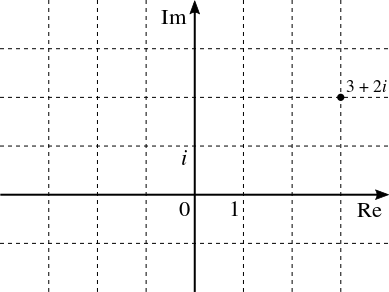
\includegraphics[width=0.21\linewidth]{images/gauss.png}
	\caption{Source:  Wikipedia}
\end{figure}

Rigorously, they are defined as the set \begin{eqnarray*}S=\{a+bi &|& a,b \in \mathbb{Z}\}. \end{eqnarray*}  

\clearpage

\subsection{Gaussian Division Problem \cite{div:1}}

\mybox{0.9\textwidth}{\begin{prob}  Find a possible quotient and remainder when we divide $z=-1+4i$ by $w=1+2i$ in $\mathbb{Z}[i]$.  \end{prob}}

To begin with, before I give a rigorous definition of division in $\mathbb{Z}[i]$, I want you to explore possible quotients and remainders. That is, with no restrictions other than sticking to the Gaussian integers, find a pair $q,r$ such that $$z=-1+4i=(1+2i)q+r=wq+r.$$   We'll discuss our findings in a few minutes!

\clearpage

Here are some examples of possible pairs $(q,r)$:

\begin{itemize}
	\item $-1+4i=(1+2i)(1)+(-2+2i)$, therefore, $(q,r)=(1, -2+2i)$.
	\item $-1+4i=(1+2i)(2)+(-3)$, therefore, $(q,r)=(2, -3)$.
	\item $-1+4i=(1+2i)(i)+(1+3i)$, therefore, $(q,r)=(i, 1+3i)$.
	\item $-1+4i=(1+2i)(-i)+(-3+5i)$, therefore, $(q,r)=(-i, -3+5i)$.
	\item $-1+4i=(1+2i)(1+i)+i$, therefore, $(q,r)=(1+i, i)$.
\end{itemize}

\clearpage

\subsection*{Summarizing in a Table}

\begin{table}[h] 
	\centering
	\begin{tabular}{l l}
		\toprule
		Quotient & Remainder \\
		\midrule
		$1$ & $-2+2i$ \\
		$2$ & $-3$ \\ 
		$i$ & $1+3i$ \\
		$-i$ & $-3+5i$ \\
		$1+i$ & $i$ \\ 
		\bottomrule
		
	\end{tabular}
	
	\caption{Division Algorithm applied to $z=-1+4i$ divided by $w=1+2i$.}
	\label{tab:div}
\end{table}

\subsection*{Magnitude} 

Now the question lies on which remainder is best. When we worked with integers, we simply had the condition $0\le r<|b|$. However, how do we compare the values of two imaginary numbers such as $-2+2i$ and $-3$?  

In order to do this, we recall the magnitude of a complex number $z=a+bi$. By definition, $$|z|=\sqrt{z\bar{z}}=\sqrt{a^2+b^2},$$ where $\bar{z}$ is the complex conjugate.  

The magnitude was also equivalent to the Euclidean distance between a point in the complex plane and the origin.

\subsection{Norms}

Since with Euclidean Domains, we want to work with integers, we define the \textbf{norm} of a complex number $z=a+bi$ to be $$N(a+bi)=z\bar{z}=a^2+b^2.$$  
The norm function is used in comparing lengths of Gaussian Integers when using the division algorithm.  

Note that the norm function over $\mathbb{Z}$ was $N(b)=|b|$.  

\clearpage

\subsection*{Making the Table Normal}


\begin{table}[h]
	\centering
	\begin{tabular}{l l l }
		\toprule
		Quotient & Remainder & Norm \\
		\midrule
		$1$ & $-2+2i$ & $8$ \\
		$2$ & $-3$ & $9$  \\ 
		$i$ & $1+3i$ & $10$ \\
		$-i$ & $-3+5i$ & $34$\\
		$1+i$ & $i$ & $\framebox{1}$ \\ 
		\bottomrule
	\end{tabular}
	\caption{Extension of Table \ref{tab:div} with Norms}
\end{table}

\clearpage

We therefore see that the best way to divide $z=-1+4i$ by $w=1+2i$ of the quotients attempted is $$z=-1+4i=(1+2i)(1+i)+i=wq+r.$$  Note that $$N(r)=1<N(w)=5.$$  

In general, the statement of the division algorithm over $\mathbb{Z}[i]$ ensures the existence and uniqueness of a pair $(q,r)$ for which  \begin{eqnarray*} z=wq+r &|& N(r)<N(w). \end{eqnarray*} 

\subsection{Visualizing Division in Gaussian Integers}

\begin{figure}[H]
	\centering\includegraphics[width=0.5\linewidth]{images/kitchings.jpg}
	\caption{Source:  Clay Kitchings \cite{div:1}}
\end{figure}

\subsection{Uniqueness} 

Note that the solution pair for $(q,r)$ is not unique. If we look at the square of points around $z$ on the diagram above, we see that $q=1+2i$ and $q=2+i$ both work.
\begin{itemize}
	\item When $q_2=1+2i$, for instance, we have $$r_2=(-1+4i)-\left(1+2i\right)\left(1+2i\right)=(-1+4i)-\left(1+4i-4\right)=2.$$
	\item When $q_3=2+i$, we have $$r_3=(-1+4i)-\left(1+2i\right)\left(2+i\right)=(-1+4i)-(2+5i-2)=-1-i.$$
\end{itemize}
Note that $N(r_2)=4<N(w)=5$ and $N(r_3)=2<N(w)=5$.

\clearpage

\section{Base Numbers}

Base numbers are the heart of computers with both binary and hexadecimal. Binary can refer to the $2$ states of a switch - on or off. Hexadecimal can be used to describe locations in computer memory or colours with HTML.  

\begin{defi} When we write numbers using the first $b$ whole numbers (i.e. $0, 1, 2, \cdots, b-1$), this is a base $b$ system.  \cite{aops:1} \end{defi}

We can think of base conversions as different ways of \textit{grouping numbers}.
\clearpage

\subsection{Binary}

The most common and applicable base is binary. In binary, the only two usable digits are $0$ and $1$. Therefore, we have to write every number as a sum of powers of $2$. 

For instance, to write $19$ in binary, we would write $$19=16+2+1=2^4+2^1+2^0=10011_2.$$  

Similarly, to convert from binary to decimal, we find the power of $2$ that each $1$ corresponds with: $$101010_2=2^5+2^3+2^1=32+8+2=42.$$  

\subsection{Base Conversion Problem}

When working with bases that are not binary, things get slightly more complicated. If we want to convert the positive number $n$ into base $b$, we use a similar algorithm to binary.  

We attempt to find the highest power of the base $b$ that goes into the number $n$. We then subtract this from the number $n$ and repeat until we get to the units digit. 

\mybox{0.8\textwidth}{\begin{prob} Convert $2016$ into base $8$.  \end{prob}}

\clearpage

\subsection{Subtracting Powers of 8}

We begin by listing powers of $8$:  $$8, 64, 512, 4096, \cdots.$$  

The largest power of $8$ that is less than $2016$ is $512$. We divide $2016$ by $512$ using the division algorithm:
$$2016=512\times 3+480.$$  

\clearpage

We then repeat the process by finding the largest power of $8$ less than $480$, $64$. We divide $480$ by $64$ using the division algorithm: $$480=64\times 7+32.$$ 
Finally, we write $32=8\times 4$.  Therefore, $$2016=3\times 512+7\times 64+4\times 8=3740_8.$$ To verify using Mathematica, we use the command BaseForm[2016,8]. 

\clearpage  

\subsection{Magic 8 Ball}

Instead of subtracting off powers of $8$, another method exists to convert $2016$ to base $8$. We can repeatedly divide by $8$ until the quotient is $0$ and look at the remainders: \begin{eqnarray*}  2016=8\cdot 252+&\textbf{0}& \\ 252=8\cdot 31+&\textbf{4}& \\ 31=8\cdot 3+&\textbf{7}& \\ 3=8\cdot 0+&\textbf{3}& \end{eqnarray*}

We append each of the remainders in \textit{backwards order} to determine $2016=3740_8$.

\clearpage

\section{Contest Style Base Number Problems}  

\mybox{0.9\textwidth}{\begin{prob} Funky base conversions. \begin{enumerate} \item Convert $25681_9$ to base $3$. \item Convert $11,101,001,111_2$ to base $8$. \end{enumerate} \end{prob} \begin{prob}[AIME 1986] The increasing sequence $1,3,4,9,10,12,13\cdots$ consists of all those positive integers which are exponent powers of $3$ or sums of distinct powers of $3$. Find the $100^{\mbox{th}}$ term of this sequence.\end{prob}}

\subsection{Funky Base Conversions}

\begin{proof}[Solution] 
We begin by writing out \begin{eqnarray*} 25681_9&=&2\cdot 9^4+5\cdot 9^3+6\cdot 9^2+8\cdot 9^1+1\cdot 9^0 \\ &=& 2\cdot \left(3^2\right)^4+5\cdot \left(3^2\right)^3+6\cdot \left(3^2\right)^2+8\cdot \left(3^2\right)^1+1\cdot \left(3^2\right)^0 \\ &=& \textbf{2}\cdot 3^8+\textbf{5}\cdot 3^6+\textbf{6}\cdot 3^4+\textbf{8}\cdot 3^2+\textbf{1}\cdot 3^0. \end{eqnarray*}

The problem we have is that in base 3, the only digits we are allowed to use are $0, 1, 2$. Therefore, what do we do about the $5, 6, 8$?  

\clearpage

We conver them all to base 3! $5=3\cdot 1+2, 6=3\cdot 2+0, 8=3\cdot 2+2$. We plug these in to the above equation: 
\begin{eqnarray*}
 25681_9 &=& \textbf{2}\cdot 3^8+\textbf{5}\cdot 3^6+\textbf{6}\cdot 3^4+\textbf{8}\cdot 3^2+\textbf{1}\cdot 3^0 \\ 
	&=& \textbf{2}\cdot 3^8+\left(3+2\right)\cdot 3^6+(3\cdot 2)\cdot 3^4+(3\cdot 2+2)\cdot 3^2+\textbf{1}\cdot 3^0 \\ 
	&=& \textbf{2}\cdot 3^8+\textbf{1}\cdot 3^7+\textbf{2}\cdot 3^6+\textbf{2}\cdot 3^5+\textbf{2}\cdot 3^3+\textbf{2}\cdot 3^2+\textbf{1}\cdot 3^0 \\
	&=& \boxed{212202201_3}.  \end{eqnarray*}

A shortcut to doing this would be converting each digit directly to base $3$ and appending the digits: $$2=2_3,\: 5=12_3,\: 6=20_3,\: 8=22_3,\: 1=01_3.$$ 

\clearpage

For problem 2, inspired by our success in the previous problem, we manipulate the sum of powers of $2$. Since $8=2^3$, we have to group the numbers in groups of $3$: \begin{eqnarray*} 11,101,001,111_2 &=& 2^{10}+2^9+2^8+2^6+2^3+2^2+2^1+2^0 \\ &=& \left(2+1\right)2^9+\left(2^2+1\right)2^6+\textbf{1}\cdot 2^3+\left(2^2+2^1+2^0\right) \\ &=& \textbf{3}\cdot 8^3+\textbf{5}\cdot 8^2+\textbf{1}\cdot 8^1+\textbf{7}\cdot 8^0 \\ &=& \boxed{3517_8}. \end{eqnarray*}

Note that as before, a shortcut exists! The commas are extra helpful here. $$11_2=3,\: 101_2=5,\: 001_2=1,\: 111_2=7.$$   \end{proof}
\clearpage

\subsection{AIME 1986}
\begin{proof}[Solution]
We begin by writing out the first few terms of the sequence as sums of distinct powers of $3$.  \begin{eqnarray*}\textbf{1}=3^0,\: \textbf{3}=3^1,\:\textbf{4}=3^1+3^0,\: \textbf{9}=3^2,\: \\ \textbf{10}=3^2+3^0,\: \textbf{12}=3^2+3^1,\: \textbf{13}=3^2+3^1+3^0,\: \cdots. \end{eqnarray*}

Does anyone notice anything interesting about the powers of $3$ used?

\clearpage


\begin{table}[h]
	\centering
	\begin{tabular}{|l | r r r|}
		\toprule
		Number in Sequence & & &\\
		                   & $3^2$ & $3^1$ & $3^0$ \\ 
		\midrule
		\textbf{1} & 0 & 0 & 1 \\
		\textbf{3} & 0 & 1 & 0 \\
		\textbf{4} & 0 & 1 & 1 \\
		\textbf{9} & 1 & 0 & 0 \\
		\textbf{10} & 1 & 0 & 1 \\
		\textbf{12} & 1 & 1 & 0 \\
		\textbf{13} & 1 & 1 & 1 \\
		\bottomrule
	\end{tabular}
	\caption{Coefficients of Powers of 3}
	\label{tab-pow3}
\end{table}


\clearpage

The numbers on the right hand of the table should look familiar!
\newline
\begin{defi}  A \textbf{bijection} is a function between two sets $X$ and $Y$ such that every element in $X$ is mapped to $Y$ and every element in $Y$ is mapped to $X$. Mathematically, we write this as $f:X\to Y$.  \end{defi}

Where is there a bijection in this problem? As a hint, each term in the sequence can either have a specific power of $3$ or not have a power of $3$. 

\clearpage

\begin{table}[h]
	\centering
	\begin{tabular}{|l|l | r r r|}
		\toprule
		Term \# & Number in Sequence & & &\\
		& & $3^2$ & $3^1$ & $3^0$ \\ 
		\midrule
		1&\textbf{1} & 0 & 0 & 1 \\
		2&\textbf{3} & 0 & 1 & 0 \\
		3&\textbf{4} & 0 & 1 & 1 \\
		4&\textbf{9} & 1 & 0 & 0 \\
		5&\textbf{10} & 1 & 0 & 1 \\
		6&\textbf{12} & 1 & 1 & 0 \\
		7&\textbf{13} & 1 & 1 & 1 \\
		\bottomrule
	\end{tabular}
	\caption{Extension of Table \ref{tab-pow3} Adding the Term Number}
\end{table}

\clearpage

There appears to be a bijection between the term number in the sequence on the left hand side and the decimal form of the binary numbers formed on the right hand side of the table! 

Now, how do we find the $100$th term in the sequence? In order to do this, we first have to convert $100$ to binary: $$100=64+32+4=2^6+2^5+2^2=1100100_2.$$  

Then, by the bijection established above, each of the $1$'s and $0$'s actually correspond to powers of $3$. Therefore, the $100$th term in the sequence is $$3^6+3^5+3^2=\boxed{981}.$$  \end{proof}



\clearpage



\section{Fundamental Theorem of Arithmetic}

In 1801, Gauss proved the Fundamental Theorem of Arithmetic in his book ``Disquisitiones Arithmeticae". 

\mybox{0.8\textwidth}{\begin{theorem} Every integer at least $2$ is either prime itself or is the unique product of primes. \end{theorem}}

This theorem is the reason $1$ is not a prime number; otherwise, the product would not be unique! Before proving the Fundamental Theorem of Arithmetic, we revisit our friend Euclid and learn about induction. 
\clearpage

\subsection{Euclid's Lemma}
\begin{displayquote} ``If two numbers by multiplying one another make some number, and any prime number measure the product, it will also measure one of the original numbers." \\ - Euclid's Elements, Book VII, Proposition 30" \end{displayquote}
In other words, if prime $p\mid ab$ for integers $a,b$, then $p\mid a$ or $p\mid b$. The proof of Euclid's Lemma requires Bezout's Theorem, which will come later in this course! 

\clearpage

%%%%%Domino effect video 
\subsection{$\star$ Induction}
Another key factor in the proof of the Fundamental Theorem of Arithmetic is the method of \textbf{mathematical induction}.
	
\begin{defi}[Induction] In order to prove a statement $P(x)$ is true for all positive integers $x\ge a$, it suffices to show this in two parts: \begin{enumerate}
		\item \textit{The base case:} $P(a)$ is true.
		\item \textit{The inductive step:} For all positive integers $k\ge a$, $P(k)$ being true implies $P(k+1)$ is also true.
		\end{enumerate}  
		This is a domino effect where one domino knocks down the next.
\end{defi}

\clearpage

\begin{figure}[h]
	\centering\includegraphics[width=0.45\linewidth]{images/induction.jpg}
	\caption{Source: Something Of That Ilk}
\end{figure}
\clearpage

For instance, suppose I wish to show the identity $$1+2+3+\cdots+n=\frac{n(n+1)}{2}$$ holds for all $n\ge 1$.
I begin by showing the identity holds for $n=1$: $1=\frac{1\cdot 2}{2}$. I then show that if the identity is true for $n=k$, then it is also true for $n=k+1$. The inductive \textit{hypothesis} is that $1+2+3+\cdots+k=\frac{k(k+1)}{2}$. We use this to show the identity holds for $n=k+1$. Indeed, note that \begin{eqnarray*} \left(1+2+3+\cdots+k\right)+k+1 &=& \frac{k(k+1)}{2}+k+1 \\ &=& (k+1)\left(\frac{k}{2}+1\right) \\ &=& \frac{(k+1)(k+2)}{2}. \end{eqnarray*}

\clearpage
\begin{defi}[Strong Induction] Replace the inductive step with: If $P(a), P(a+1), P(a+2), P(a+3), \cdots, P(k-1), P(k)$ being true \textit{implies} that $P(k+1)$ is also true.  \end{defi} The way I visualize strong induction is below:
\begin{eqnarray*} P(a)&\implies& P(a+1) \\ 
				 P(a)\:, P(a+1) &\implies& P(a+2) \\
				 P(a)\:, P(a+1), P(a+2) &\implies& P(a+3) \\
				 \cdots
\end{eqnarray*}
It is a slightly more confusing domino effect! Knowing strong induction will be particularly useful when you take an analysis class down the road.
\clearpage
\subsection{$\star$ Proof}
While the notation may be confusing now, after we see strong induction in action, it will make more sense!

\begin{theorem} Every integer at least $2$ is either prime itself or is the unique product of primes. \end{theorem}

\begin{proof} We prove the Fundamental Theorem of Arithmetic. There are two parts for the proof: showing the existence of a prime factorization, and the uniqueness of the prime factorization. We begin with the \color{blue} existence part.  
	
\clearpage
	
\color{black} We use the method of strong induction. We desire to show that all positive integers greater than or equal to $2$ are either prime or can be expressed as the product of primes. To begin with, as a \color{ForestGreen} base case, \color{black} $2$ itself is prime. 

Furthermore, using the \color{ForestGreen} strong induction hypothesis, \color{black} assume that we have proven the the existence of a prime factorization for all integers $y$ with $2\le y\le k$. We then prove the existence for $k+1$. We have two cases to consider: either $k+1$ is prime, or it is the product of two numbers $a,b$ greater than $1$.

If $k+1$ itself is prime, then this satisfies the first condition of the Fundamental Theorem of Arithmetic. Otherwise, $k+1=ab$. 

By the strong induction hypothesis, since $2\le a,b<k+1$, \color{black} both $a$ and $b$ are the product of primes. Therefore, $k+1$ is also the product of primes.

By the method of strong induction, we have proved the existence of a prime factorization. We now go about proving uniqueness. 

For the \color{blue} uniqueness part\color{black}, we use proof by contradiction. Consider the set $S$ of positive integers that do not have a unique prime factorization. I will show that $S$ must be empty by assuming for the sake of contradiction that $S$ is non-empty.

Then, using the well-ordering principle, $S$ must have a least element, say $n$. Let the two possible prime factorizations of $n$ be $$n=p_1p_2p_3\cdots p_s=q_1q_2q_3\cdots q_r.$$ I will show that there is a smaller value in $S$ than $n$, contradicting its minimality.  

We see that $p_1\mid q_1q_2q_3\cdots q_r$. By Euclid's Lemma, we must have $p_1\mid q_j$ for some $1\le j\le r$. However, since they are primes, this implies that $p_1=q_j$. We cancel out this similar term to get $$\frac{n}{p_1}=\frac{n}{q_j}=p_2p_3\cdots p_s=q_1q_2q_3\cdots q_{j-1}q_{j+1}\cdots q_r.$$ 

Therefore, we have shown that $\frac{n}{p_1}=\frac{n}{q_j}$ does not have a unique prime factorization! This contradicts the minimality of $n$, and the set $S$ must be empty.  \end{proof}

What does Gauss' proof of the Fundamental Theorem of Arithmetic imply? It allows us to write numbers in their prime factorization. For instance, $120=2^3\cdot 3\cdot 5$ and $182=2\cdot 7\cdot 13$. 

While the proof may seem very complicated at first, seeing induction proofs is very important for higher level mathematics. The statement of induction and the well-ordering principle are actually equivalent! For more information on proofs, see my lecture to Northern Nevada Math, \color{Orange}\href{https://numbertheoryguydotcom.files.wordpress.com/2016/03/intermediateproofs.pdf}{Intermediate Proofs.}

\clearpage

\subsection{Canonical Prime Factorization}

\color{black} The preferred method for writing the prime factorization of a positive integer $n$ is $$n=\prod_{j=1}^{k}\left(p_j^{e_j}\right)=p_1^{e_1}p_2^{e_2}\cdots p_k^{e_k}.$$ 
The $\prod$ symbol is similar to the $\sum$ symbol, except we multiply all the terms!

Writing prime factorizations in this form makes it easier to compute the gcd and lcm of two numbers. It also allows us to do many problems involving divisors!

\section{Applications of the Fundamental Theorem of Arithmetic}

\subsection{GCD and LCM}
For two positive integers $a$ and $b$, we write out their prime factorizations: $$a=p_1^{a_1}p_2^{a_2}\cdots p_k^{a_k}, b=p_1^{b_1}p_2^{b_2}\cdots p_k^{b_k}.$$ Then, \begin{eqnarray*} \gcd(a,b)&=&p_1^{\min(a_1, b_1)}p_2^{\min(a_2, b_2)}\cdots p_k^{\min(a_k, b_k)} \\ \lcm[a,b]&=&p_1^{\max(a_1, b_1)}p_2^{\max(a_2, b_2)}\cdots p_k^{\max(a_k, b_k)}. \end{eqnarray*}
\clearpage

For instance, when $a=2^6\cdot 3^5\cdot 7^2$ and $b=2^9\cdot 3^1\cdot 7^0$, then \begin{eqnarray*} \gcd(a,b)=2^{\min(6,9)}\cdot 3^{\min(5,1)}\cdot 7^{\min(2,0)}=2^6\cdot 3^1\cdot 7^0 \\ \lcm[a,b]=2^{\max(6,9)}\cdot 3^{\max(5,1)}\cdot 7^{\max(2,0)}=2^9\cdot 3^5\cdot 7^2. \end{eqnarray*}

Note that $\gcd(a,b)\lcm[a,b]=2^{6+9}\cdot 3^{1+5}\cdot 7^2=ab$. This is true in general because $\min(a_j, b_j)+\max(a_j, b_j)=a_j+b_j$. 

\clearpage

\subsection{Tau and Sigma}

\begin{defi} Define $\tau(n)$ to be the number of positive divisors of $n$ and $\sigma(n)$ to be the sum of the positive divisors of $n$. For instance, for $n=12$, its divisors are $1, 2, 3, 4, 6, 12$. Therefore, $\tau(12)=6$ and $\sigma(12)=1+2+3+4+6+12=28$. \end{defi}

\mybox{0.8\textwidth}{\begin{prob} If $n=144$, find the number of positive divisors of $n$ and the sum of the positive divisors of $n$. Is there a fast method? Compute $\tau(4800)$ and $\sigma(4800)$. What about general $n$? \end{prob}}

\clearpage

\begin{proof}[Solution]

For $n=144$, we list the positive divisors: $$\{1, 2, 3, 4, 6, 8, 9, 12, 16, 18, 24, 36, 48, 72, 144\}.$$ We see that there are $\tau(144)=15$ divisors by counting. We can also take the sum of all the divisors by hand to get $\sigma(144)=403$. However, listing the divisors method will not work for larger values of $n$. 

Therefore, we attempt to factorize $n$: $144=2^4\cdot 3^2$. Note that all divisors of $n$ must be of the form $d=2^{a}\cdot 3^{b}$. Remembering our $v$ notation, another way of writing this is $v_2(d)=a$ and $v_3(d)=b$.   

\color{ForestGreen} We must have $0\le a\le 4$ and $0\le b\le 2$. \color{black} Otherwise, it wouldn't be possible for $d$ to divide into $n$, since there would either be too many $2$'s or $3$'s.  

\clearpage

Therefore, we have $4+1=5$ choices for $a$: $0,1,2,3,4$. Similarly, we have $2+1=3$ choices for $b$. Since our choices for $a$ and $b$ are independent of one another, there is a total of $\sigma(144)=5\cdot 3=\boxed{15}$ positive divisors. 

What about the sum of the divisors of $144$? I claim that the product $(1+2+2^2+2^3+2^4)(1+3+3^2)$ is the sum of the divisors of $144$. One way to see this is multiplying the product: \color{red} \footnotesize \begin{eqnarray*}  1\left(1+3+3^2\right)+\:2\left(1+3+3^2\right)+\: 2^2\left(1+3+3^2\right)+\:2^3\left(1+3+3^2\right)+\:2^4\left(1+3+3^2\right) \end{eqnarray*} \normalsize\color{black} From this distribution, how do I get all possible divisors of $144$?  

\clearpage
\begin{eqnarray*} 1\left(1+3+3^2\right)&=& 1+3+9 \\ 2\left(1+3+3^2\right)&=& 2+6+18 \\ 2^2\left(1+3+3^2\right)&=&4+12+36 \\ 2^3\left(1+3+3^2\right)&=&8+24+72 \\ 2^4\left(1+3+3^2\right)&=&16+48+144. \end{eqnarray*}

Our original list of divisors was $\{1, 2, 3, 4, 6, 8, 9, 12, 16, 18, 24, 36, 48, 72, 144\}$. We see that every divisor is included in the sum! 

\clearpage

A faster method to see this is to choose an arbitrary divisor of $144$, say $24$. Note that $24=2^3\cdot 3$. Therefore, we colour the two terms of the product which multiply to $24$. $$\left(1+2+2^2+\color{blue}2^3\color{black}+2^4\right)\left(1+\color{blue}3\color{black}+3^2\right).$$  
Hence, by the distributive property, $24$ is a part of our sum.

This logic extends to all divisors of $144$, since they are of the form $2^a3^b$ mentioned above! Note that $1+2+2^2+2^3+2^4=31$ and $1+3+3^2=13$, hence the sum of the positive divisors is $\sigma(144)=31\cdot 13=\boxed{403}$.

Next, we compute $\tau(4800)$ and $\sigma(4800)$. Using the method we developed above, we begin by factorizing $4800$: $4800=2^6\cdot 3^1\cdot 5^2$. Therefore, all positive divisors are of the form \begin{eqnarray*}\{2^a\cdot 3^b\cdot 5^c &|& 0\le a\le 6,\:\: 0\le b\le 1,\:\: 0\le c\le 2\}. \end{eqnarray*}
Therefore, we have $7$ choices for $a$, $2$ for $b$, and $3$ for $c$, for a total of $\tau(4800)=7\cdot 2\cdot 3=\boxed{42}$ divisors.

To compute the sum of the divisors, we compute a similar product:  $$\sigma(4800)=(1+2+2^2+2^3+2^4+2^5+2^6)(1+3^1)(1+5+5^2)=\boxed{15,748}.$$ 
\clearpage

\mybox{0.95\textwidth}{\begin{theorem}[Tau and Sigma] If $n$ is a positive integer with $k$ prime factors and canonical prime factorization $\displaystyle n=\prod_{j=1}^{k}\left(p_j^{e_j}\right)=p_1^{e_1}p_2^{e_2}\cdots p_j^{e_j},$ then \begin{eqnarray*} \tau(n)&=&\prod_{j=1}^{k}\left(e_j+1\right) \\ \sigma(n)&=&\prod_{j=1}^{k}\left(p_j^0+p_j^1+p_j^2+\cdots+p_j^{e_j}\right)=\prod_{j=1}^{k}\left(\sum_{e=0}^{e_j}p_j^{e}\right),  \end{eqnarray*} where $\tau(n)$ is the number of positive divisors of $n$ and $\sigma(n)$ is the sum. \end{theorem}}

\subsection*{Turning Symbols into Language}
Remember that $\prod$ is the symbol for multiplying terms and $\sum$ is the symbol for adding terms. Therefore, the first expression is $$\tau(n)=\prod_{j=1}^{k}\left(e_j+1\right)=\left(e_1+1\right)\left(e_2+1\right)\cdots \left(e_k+1\right).$$ Since $\tau(n)$ counts the number of positive divisors of $n$, let $d$ be an arbitrary divisor. As established by our work above, for a prime $p_j$ in our prime factorization of $n$, $0\le v_{p_j}(d)\le e_j$. Therefore, there are $e_j+1$ choices for the exponent of $p_j$. We multiply these to determine our formula for $\tau(n)$. \end{proof}
\clearpage

  
\subsection{Jail Puzzle}

\mybox{0.8\textwidth}{\begin{prob} The cells in a jail are numbered from $1$ to $100$ and their doors are activated from a central button.  The activation opens a closed door and closes an open door.  Starting with all the doors closed the button is pressed $100$ times.  When it is pressed the $k$-th time the doors that are multiples of $k$ are activated.  Which doors will be open at the end? \end{prob}}

\clearpage

\begin{figure}[h]
	\centering\includegraphics[width=0.9\linewidth]{images/jail.jpg}
	\caption{Source: Knepfle.com}
\end{figure}

\subsection*{Let's Press the Button!}
\begin{proof}[Solution]
One problem solving trick when we don't know how to begin a problem is to simplify the problem. The number $100$ seems arbitrary; therefore, we try the problem for a jail with $10$ cells. We create a table of which jail cells are activated each time we press the button.

In the table, the jail cells are represented by the columns and the button pressing is represented by the rows. Note that a jail cell will be open at the end if it is activated an odd number of times, because it begins even. Therefore, we sum up the number of check marks for each jail cell in the button row, and if it is odd, we highlight it green.

\clearpage

\begin{table}[h]
	\centering %nice job Justin!
	\scalebox{0.9}{
		\begin{tabular}{|l | r r r r r r r r r r|}
			\toprule
			Button \# & 1 & 2 & 3 & 4 & 5 & 6 & 7 & 8 & 9 & 10 \\
			\midrule
			1 & \checkmark & \checkmark & \checkmark & \checkmark & \checkmark & \checkmark & \checkmark & \checkmark & \checkmark & \checkmark \\
			2 & \x & \checkmark & \x & \checkmark & \x & \checkmark & \x & \checkmark & \x & \checkmark \\
			3 & \x & \x & \checkmark & \x & \x & \checkmark & \x & \x & \checkmark & \x \\
			4 & \x & \x & \x & \checkmark & \x & \x & \x & \checkmark & \x & \x \\
			5 & \x & \x & \x & \x & \checkmark & \x & \x & \x & \x & \checkmark \\
			6 & \x & \x & \x & \x & \x & \checkmark & \x & \x & \x & \x \\
			7 & \x & \x & \x & \x & \x & \x & \checkmark & \x & \x & \x \\
			8 & \x & \x & \x & \x & \x & \x & \x & \checkmark & \x & \x \\
			9 & \x & \x & \x & \x & \x & \x & \x & \x & \checkmark & \x \\
			10& \x & \x & \x & \x & \x & \x & \x & \x & \x & \checkmark \\ \midrule
			 & \color{ForestGreen}1\color{black} & 2 & 2 & \color{ForestGreen}3\color{black} & 2 & 4 & 2 & 4 & \color{ForestGreen}3\color{black} & 4 \\ 
			\midrule
	\end{tabular}}
\end{table}

\clearpage

Therefore the jail cells which are open will be cells $1, 4, 9$. Note that these are all perfect squares! Furthermore, the bottom column appears to be the number of divisors of the jail cell. For instance, $\tau(6)=4$.  Why is this the case?

A jail cell $j$ will be activated when the button is pressed the $k$-th time if and only if $k$ divides $j$. Therefore, the number of times it is activated is equivalent to the number of positive divisors of $j$, or $\tau(j)$.

Hence, the problem reduces down to when $\tau(j)$ is odd!

\clearpage

If $j$ has a prime factorization of $j=p_1^{e_1}p_2^{e_2}\cdots p_k^{e_k}$, then by our formula, $\tau(j)=\prod (e_i+1)$. If $\tau(j)$ is odd, then each term in the product must be odd. Therefore, $e_i$ must be even! Hence, every exponent in the prime factorization of $j$ is even, and $j$ must be a perfect square.

Therefore, for our original problem with $100$ doors, the doors that are open at the end are: $$1, 4, 9, 16, 25, 36, 49, 64, 81, 100.$$  \end{proof}

	


\section{Contest Style Fundamental Theorem Problems}

\mybox{0.9\textwidth}{\begin{prob}[AHSME 1996] If $n$ is a positive integer such that $2n$ has $28$ positive divisors and $3n$ has $30$ positive divisors, then how many positive divisors does $6n$ have? \end{prob} \begin{prob} Find the number of ordered triples $(x,y,z)$ for which $xyz=2400$ over the positive integers.  \end{prob}}

\clearpage
\subsection{AHSME 1996}
\begin{proof}[Solution] We focus on the condition that $2n$ has $28$ positive divisors. For primes $p, q, r$, we write out possible prime factorizations of $2n$ based on its number of divisors: $2n= p^{27},\: p^{13}q,\: p^6q^3,\: p^6qr.$ We check to see when it's possible for $\tau(3n)=30$.

\begin{itemize} 
\item If $2n=p^{27}$, since $n$ must be a positive integer, we have $p=2$ and $n=2^{26}$. Then, $3n=2^{26}3^1\implies \tau(3n)=27\cdot 2=54.$ 

\item If $2n=p^{13}q$, then we either have $p=2$ or $q=2$.\\ \color{blue} When $p=2$\color{black}, then $n=2^{12}q$, giving $$3n=2^{12}3^1q.$$ If $q=3$, then $\tau(3n)=\tau(2^{12}3^2)=(12+1)(2+1)=39$. \\ If $q\neq 3$, then $\tau(3n)=\tau(2^{12}3^1q)=(12+1)(1+1)(1+1)=52.$ \\ \\ \color{blue} When $q=2$\color{black}, we have $n=p^{13}$ and $3n=3^1p^{13}$. \\ If $p=3$, then $\tau(3n)=\tau(3^{14})=14+1=15$. \\ If $p\neq 3$, then $\tau(3n)=\tau(3^1p^{13})=(1+1)(13+1)=28$. 
\clearpage

\item If $2n=p^6q^3$, then once again, we divide this into the cases $p=2$ and $q=2$. \\  \color{blue} When $p=2$\color{black}, we have $n=2^5q^3$ and $3n=2^53^1q^3$. \\
\color{ForestGreen} If $q=3$, then $\tau(3n)=\tau(2^5\cdot 3^4)=(5+1)(4+1)=30$. \\
\color{black} If $q\neq 3$, then $\tau(3n)=\tau(2^53^1q^3)=(5+1)(1+1)(3+1)=48$.
\end{itemize}
We could continue on with the casework to verify that $n=2^53^3$ is the only solution, however, it's not particularly illuminating, therefore, I leave it as an exercise.

To conclude the problem, $6n=2^63^4$, then $\tau(6n)=\left(6+1\right)\left(4+1\right)=\boxed{35}$. \end{proof}

\clearpage

\subsection{Ordered triples with $xyz=2400$ over $\mathbb{Z}^{+}$.}

We begin by prime factorizing $480=2^5\cdot 3^1\cdot 5^2$. We write $$x=2^{x_2}3^{x_3}5^{x_5};\: y=2^{y_2}3^{y_3}5^{y_5};\: z=2^{z_2}3^{z_3}5^{z_5}.$$ Since $xyz=480$, this is equivalent to having \begin{eqnarray*} x_2+y_2+z_2 &=& 5 \\ x_3+y_3+z_3&=&1 \\ x_5+y_5+z_5&=&2. \end{eqnarray*}
How many integer triplets can you find for $(x_2, y_2, z_2)$?
\clearpage

We could begin listing possible triplets, but there are far too many to list. Therefore, we try to think of a clever method. We use a method in combinatorics known as \textbf{stars and bars}. We create a bijection between the number of ordered triplets $(x_2, y_2, z_2)$ and the rearrangement of stars and bars.

We desire to distribute $5$ $1's$ to three variables. Therefore, we write out the $5$ $1's$ as such: $1\: 1\: 1\: 1\: 1.$ We desire to divide this into three groups, therefore, we place two dividers, which we symbolize by \color{blue} blue $x$'s: \color{black} $$\mathlarger{1}\:\color{blue}x\color{black}\: \mathlarger{1}\:\: \mathlarger{1}\:\color{blue}x\color{black}\: \mathlarger{1}\:\: \mathlarger{1}\:$$ What is $(x_2, y_2, z_2)$ with these dividers?
\clearpage
$$\mathlarger{1}\:\color{blue}x\color{black}\: \mathlarger{1}\:\: \mathlarger{1}\:\color{blue}x\color{black}\: \mathlarger{1}\:\: \mathlarger{1}\:$$In the above configuration, we have $(x_2, y_2, z_2)=(1,2,2)$, since there is one $1$ in the first group and two $1$'s in the other two groups. 

In order to find the number of possible triplets $(x_2, y_2, z_2)$, we find the number of rearrangements of the objects above. The number of ways to order the $1$'s and $\color{blue} x\color{black}$'s is $\binom{7}{2}=\frac{7\cdot 6}{2}=\color{orange} 21$. \color{black}

Since $x_3+y_3+z_3=1$, we note that there are \color{orange} $3$ \color{black} possible triplets for $(x_3, y_3, z_3)$, depending on which of the variables we choose to give the $1$ to.

\clearpage

Finally, for $(x_5, y_5, z_5)$, we use the stars and bars trick again. We have the same configuration as above, except, only two $1$'s: $$\mathlarger{1}\:\color{blue}x\color{black}\: \mathlarger{1}\:\: \color{blue}x\color{black}\:$$In the example above, $(x_5, y_5, z_5)=(1, 1, 0)$. There are $\binom{4}{2}=\color{orange}6\color{black}$ rearrangements.

Therefore, in conclusion, there are $\color{orange} 21 \color{black}$ triplets for $(x_2, y_2, z_2)$, $\color{orange} 3 \color{black}$ triplets for $(x_3, y_3, z_3)$, and $\color{orange} 6 \color{black}$ triplets for $(x_5, y_5, z_5)$. Hence, the number of ordered triplets is $21\cdot 3\cdot 6=\boxed{378}$.

\clearpage

\subsection{Least Common Multiples}
\mybox{0.8\textwidth}{\begin{prob}[AIME 1998]  For how many values of $k$ is $12^{12}$ the least common multiple of $6^6$, $8^8$, and $k$?  \end{prob} \begin{prob} Let $[r,s]$ denote the least common multiple of positive integers $r$ and $s$.  Find the number of ordered triples $a,b,c$ such that $[a,b]=1000, [b,c]=2000, [c,a]=2000$. \end{prob}}

\subsection{AIME 1998}

We find the prime factorizations of these numbers. We have $$12^{12}=2^{24}\cdot 3^{12}, 6^6=2^6\cdot 3^6 \text{ and } 8^8=2^{24}.$$ Let $k=2^{k_1}3^{k_2}$.  We then rewrite the equation as $$\lcm[2^6\cdot 3^6\:, 2^{24}\:, 2^{k_1}3^{k_2}]=2^{24}\cdot 3^{12}.$$ Since none of the first two terms have a factor of $3^{12}$, we must have $k_2=12$. 

On the other hand, the second term has a factor of $2^{24}$. Therefore, we must have $0\le k_1\le 24$, giving $\boxed{25}$ possible values of $k$.  
\subsection{AIME 1987}

Notice that $1000=2^3\times 5^3, 2000=2^4\times 5^3$.  Since we are working with least common multiples, set $$a=2^{a_1}5^{a_2}, b=2^{b_1}5^{b_2}, c=2^{c_1}5^{c_2}.$$
By looking at the exponent of $2$, we see that $v_2([a,b])=3$ and $v_2([b,c])=v_2([c,a])=4$.
If $a_1$ or $b_1$ were greater than $3$, then the first equation would be false. Therefore, we must have $\color{blue} a_1, b_1\le 3$, and \color{ForestGreen} at least one of them must be equal to $3$. \color{black} Further, for the second two relations to be true, we must have $\color{blue} c_1=4$.  

Now, we consider the powers of $5$. We note that $v_5([a,b])=3, v_5([a,c])=3, v_5([b,c])=3$. This gives us four separate cases, whena ll of the numbers are $3$ or when two of them are, while the third is less than $3$: $$(a_2, b_2, c_2)=(3,3,3), (3,3,x), (3,x, 3), (x,3,3).$$ We know that $0\le x\le 2$, therefore, there are $3$ possibilities for each of the $x$'s above. Hence, there are a total of $3\cdot 3+1=10$ possibilities for the power of $5$.

In conclusion, there is a total of $7\cdot 10=\boxed{70}$ ordered triples $a,b,c$ which work.  
\clearpage

\section{Modular Arithmetic}

Modular Arithmetic is incredibly powerful and is used in cryptography, computer science, chemistry, music, and many other places. In the below picture, if $45$ hours elapse, where would the hour hand be?

\begin{figure}[h]
	\centering\includegraphics[width=0.2\linewidth]{images/clock.jpg}
	\caption{Source: Study.com}
\end{figure}

\clearpage
After $12$ hours, we see the hour hand is in the same place. Therefore, we subtract $12$ from $45$ to get $45-12=33$ hours remaining. We repeat by subtracting off $12$ hours twice more to get $33-12=21$ hours and $21-12=\boxed{9}$ hours. The numbers that the clock hand pass through each cycle of $12$ are said to be \textbf{congurent} mod $12$.
\begin{defi} We say that two integers $a$ and $b$ are equivalent modulo $n$ if and only if $n$ divides $a-b$. We write this as $a\equiv b\pmod{n}$. In the above example, $45\equiv 33\equiv 21\equiv 9\pmod{12}$. If $a\equiv b\pmod{n}$, then for positive integer $c$, several important properties are $$a+c\equiv b+c\pmod{n}, \: \:\:  \:\: \: ac\equiv bc\pmod{n}, \:\: \:  \:\:\: a-c\equiv b-c\pmod{n}.$$ 
 \end{defi} 
\clearpage


Note that in our discussion of the \color{blue}division algorithm\color{black}, $a=bq+r$ is equivalent to $a\equiv r\pmod{b}$. Furthermore, in our discussion of \color{blue} base numbers\color{black}, if $n=\left(a_ka_{k-1}\cdots a_1a_0\right)_b$, then $n\equiv a_0\pmod{b}$. 

\begin{defi} We define the set of integers $\{0, 1, 2, 3, \cdots, n-1\}$ to be the \textit{least residue system modulo} $n$. Another way of writing this system is as $\mathbb{Z}_{n}$. \end{defi} 

When a problem says to compute the value of $x$ mod $m$, we desire to find a value $y$ in our least residue system such that $x\equiv y\pmod{m}$. 

For instance, if a problem says to compute $12$ mod $5$, the answer would be $2$.

\clearpage

\subsection{Exponentiation}
For integers $a, b$ with $a\equiv b\pmod{m}$ and positive integer $e$, we have $\color{blue} a^{e}\equiv b^{e}\pmod{m}\color{black}$. For instance, to compute $6^{100}\pmod{5}$, we use the fact that $6\equiv 1\pmod{5}$ to get $6^{100}\equiv 1^{100}\equiv 1\pmod{5}.$ 
	
In several exponentiation problems, it is useful to experiment a bit. For instance, if I desired to compute $2^{100}\pmod{7}$, I would begin by computing the first few powers of $2$ mod $7$. Notice that $2^1\equiv 2\pmod{7},\: 2^2\equiv 4\pmod{7},\: 2^3\equiv 8\equiv 1\pmod{7}.$ Therefore, $$2^{100}=\left(2^3\right)^{33}\cdot 2^1\equiv 1^{33}\cdot 2^1\equiv 2\pmod{7}.$$

\clearpage
\mybox{0.8\textwidth}{\begin{prob} Use the properties of mods to calculate the following: \begin{enumerate}
			\item $\left(1+2+3+\cdots+102\right)\pmod{13}$.
			\item $64\cdot 124\pmod{7}$.
			\item $10^{100}\pmod{11}$.
			\item The units digit of $8^{5^{24}}$.
			\item $5^{70}\pmod{31}$.
\end{enumerate}
\begin{itemize}[label=$\star$]
			\item $7^{50}\pmod{43}$. 
\end{itemize}
\end{prob}}

\subsection{Solution to Examples}
\begin{enumerate}
	\item We begin by using the formula for the sum of the first $n$ positive integers: \begin{eqnarray*} 1+2+3+\cdots+102 &=& \frac{102\cdot 103}{2}=61\cdot 103. \end{eqnarray*}Next, note $51\equiv 12\equiv -1\pmod{13}$ and $103\equiv 12\equiv -1\pmod{13}$. 
	Therefore, their product is $51\cdot 103\equiv (-1)(-1)\equiv 1\pmod{13}$. 
	
	Given the simplicity of our answer, we suspect that a faster method exists.
\clearpage
	We group the sum into sets with $13$ integers: $$\{1,2,3,\cdots, 13\}, \{14, 15, 16, \cdots, 26\}, \cdots, \{79,80,81,\cdots,91\}.$$The sum of each of these set are congruent mod $13$ since each set is the result of adding $13$ to the elements of the previous set. Furthermore, because $1+2+3+\cdots+13=\frac{13\cdot 14}{2}=13\cdot 7\equiv 0\pmod{13},$ each set has sum \color{ForestGreen} $0$ mod $13$. \color{black}
	
	The final set with $13$ elements should be $\{92, 93, 94, \cdots, 103, 104\}$, however, we are \color{blue} missing the terms $103$ and $104$ in our sum\color{black}. Since the sum of this final set is also $0$ mod $13$, we have $$1+2+3+\cdots+102\equiv 0-103-104\equiv 0-12\-0\equiv 1\pmod{13}.$$ 
\clearpage
	\item We note that $64\equiv 1\pmod{7}$ since $63=9\cdot 7$ and $124\equiv 5\pmod{7}$ since $119=7\cdot 17$. Therefore, $64\cdot 124\equiv 1\cdot 5\equiv \boxed{5}\pmod{7}.$
	\item Note that $10^{100}\equiv \left(-1\right)^{100}\equiv 1\pmod{11}.$
	\item Finding the units digit of $8^{24}$ is equivalent to calculating $8^{24}$ mod $10$. We try to find a pattern. We create a table, noting that $8^2=64\equiv 4\pmod{10}, 8^3=8^2\cdot 8\equiv 4\cdot 8\equiv 2\pmod{10}, \cdots$. We attempt to see if the powers of $8$ will cycle mod $10$.
	\clearpage 
	\begin{table}[H]
		\centering
		\begin{tabular}{l r}
			\toprule
			$n$ & $8^n$ mod $10$ \\
			\midrule
			1 & 8\\
			2 & 4 \\ 
			3 & 2 \\
			4 & 6 \\
			5 & 8 \\
			6 & 4 \\
			7 & 2 \\
			$\vdots$ & $\vdots$  \\
			\bottomrule
		\end{tabular}
		\caption{Powers of $8$ mod $10$.}
	\end{table}
	\clearpage
	We see that the powers of $8$ cycle with \textbf{period} 4. Therefore, we must now compute the exponent mod $4$: $5^{24}\equiv 1^{24}\equiv 1\pmod{4}$. Therefore, in conclusion, $$8^{5^{24}}\equiv 8^{1}\equiv 8\pmod{10}.$$ 
	\item We use the same method as before by computing the first few powers of $5$ mod $31$. Note that $5^2\equiv 25\pmod{31}$ and $5^3\equiv 125\equiv 1\pmod{31}$ since $125=31\cdot 4+1$. Therefore, $$5^{70}\equiv \left(5^3\right)^{23}\cdot 5^1\equiv 5^1\equiv \boxed{5}\pmod{31}.$$
\end{enumerate}
\begin{itemize}[label=$\star$]
	\item The key insight in this problem is noting that $$7^3+1=344=43\cdot 8\equiv 0\pmod{43}.$$Hence, $7^3\equiv -1\pmod{43}$ and $7^6\equiv \left(7^3\right)^2\equiv (-1)^2\equiv 1\pmod{43}.$ We now use this for $7^{50}$: $$7^{50}\equiv \left(7^6\right)^8\cdot 7^2\equiv 49\equiv \boxed{6}\pmod{43}.$$
\end{itemize}

We have seen addition, multiplication, and subtraction with mods. However, what about division? If we wish to divide by $a$ in $\mathbb{Z}_{m}$ we must find the \textbf{inverse} of $a$ mod $m$. This is the value $x$ that solves the \textbf{linear congruence} $ax\equiv 1\pmod{m}$. In order to see when this condition can be satisfied, we look at multiplication tables. 
\clearpage 
\subsection{Multiplication Tables}

	\begin{table}[H]
	\centering
	\begin{tabular}{l | l l l l l l l}
		\toprule
		$\times$ & 0 & 1 & 2 & 3 & 4 & 5 & 6\\
		\midrule
		0 & 0 & 0 & 0 & 0 & 0 & 0 & 0 \\
		1 & 0 & 1 & 2 & 3 & 4 & 5 & 6\\ 
		2 & 0 & 2 & 4 & 6 & 1 & 3 & 5\\
		3 & 0 & 3 & 6 & 2 & 5 & 1 & 4\\
		4 & 0 & 4 & 1 & 5 & 2 & 6 & 3\\
		5 & 0 & 5 & 3 & 1 & 6 & 4 & 2 \\
		6 & 0 & 6 & 5 & 4 & 3 & 2 & 1 \\
		\bottomrule
	\end{tabular}
	\caption{Multiplication Table Mod $7$.}
\end{table}

\mybox{0.9\textwidth}{\begin{prob} From the table above, solve the linear congruences $3x\equiv 1\pmod{7}$ and $2y\equiv 1\pmod{7}$. Does division work in mod $7$?\end{prob}}
\begin{proof}[Solution] We see from the table that $3\cdot 5=15\equiv 1\pmod{7}$, hence $x\equiv 5\pmod{7}$. Furthermore, $2\cdot 4=8\equiv 1\pmod{7}$, hence $y\equiv 4\pmod{7}$. Every non-zero number in the table above has an inverse, therefore, we have division by non-zero elements in $\mathbb{Z}_7$. \end{proof}

For every prime $p$, it can be proven that we can have division by non-zero elements in $\mathbb{Z}_p$. What about a case when $p$ is not prime?

\clearpage
	\begin{table}[H]
	\centering
	\begin{tabular}{l | l l l l l l}
		\toprule
		$\times$ & 0 & 1 & 2 & 3 & 4 & 5 \\
		\midrule
		0 & 0 & 0 & 0 & 0 & 0 & 0 \\
		1 & 0 & 1 & 2 & 3 & 4 & 5 \\ 
		2 & 0 & 2 & 4 & 0 & 2 & 4 \\
		3 & 0 & 3 & 0 & 3 & 0 & 3 \\
		4 & 0 & 4 & 2 & 0 & 4 & 2 \\
		5 & 0 & 5 & 4 & 3 & 2 & 1 \\
		\bottomrule
	\end{tabular}
	\caption{Multiplication Table Mod $6$.}

\end{table}
Are there any values $x$ such that $2x\equiv 1\pmod{6}$? 
\clearpage
No! We see from the table above that we can only have $2x\equiv 0, 2, 4\pmod{6}$. The reason that $2^{-1}$ mod $6$ does not exist is because $\gcd(2,6)=2\neq 1$. Therefore, division does not exist in $\mathbb{Z}_6$.

For \color{blue}algebraic structures\color{black}, a topic of abstract algebra, we say that $\mathbb{Z}_{m}$ for composite $m$ is a \textbf{\color{red}ring\color{black}} because the elements are not invertible, and that $\mathbb{Z}_{p}$ for prime $p$ is a \textbf{\color{red}field\color{black}}.  

The above discussion is very important to two theorems in number theory: Fermat's little theorem and Euler's totient theorem. We begin by further exploring $\mathbb{Z}_{p}$.
\clearpage


\section{Fermat's Little Theorem} Pierre de Fermat (1607-1665) was a French mathematician who helped develop differential calculus, number theory, analytical geometry, and probability. In the year 1640, he stated a very important `little' theorem.

\begin{figure}[h]
	\centering\includegraphics[width=0.23\linewidth]{images/fermat.jpg}
\end{figure}


\clearpage

\subsection{Exploring Numbers}

\mybox{0.85\textwidth}{\begin{prob} Begin with the set $\{1,2,3,4,5,6\}$. Multiply each number in the set by $3$ and reduce mod $7$. What is the new set that we get? What can we say about the products of each of the two sets? \\ \\ Try to do the same thing when we multiply the set $\{1,2, 3, 4, 5, 6, 7, 8, 9, 10\}$ by $5$ and reduce mod $11$. Can we generalize? Discuss at your tables! \end{prob}}
\clearpage

	\begin{table}[H]
	\centering
	\begin{tabular}{|l | c|}
		\toprule
		$x$ & $3x\mod{7}$\\
		\midrule
		1 & 3 \\
		2 & 6 \\
		3 & 2 \\
		4 & 5 \\
		5 & 1 \\
		6 & 4 \\
		\bottomrule
	\end{tabular}
	\end{table}
We note that the two sets are the same mod $7$. Hence $$3\times \{1,2,3,4,5,6\}\equiv \{1,2,3,4,5,6\}\pmod{7}.$$
\clearpage
Since the sets are the same, their product must be the same also: \begin{eqnarray*} \left(3\times 1\right)\left(3\times 2\right)\left(3\times 3\right)\left(3\times 4\right)\left(3\times 5\right)\left(3\times 6\right)&\equiv& 6!\pmod{7} \\ 3^6\cdot 6!&\equiv& 6!\pmod{7} \\ \color{blue}3^6&\color{blue}\equiv&\color{blue} 1\pmod{7}. \end{eqnarray*}

The last step follows from the fact that $\gcd(6!, 7)=1$. 

Is this a coincidence that multiplying a set by an integer and reducing mod $p$ gives back the same set? Let's try for $p=11$.

\clearpage

	\begin{table}[H]
	\centering
	\begin{tabular}{|l | c|}
		\toprule
		$x$ & $5x\mod{11}$\\
		\midrule
		1 & 5 \\
		2 & 10 \\
		3 & 4 \\
		4 & 9 \\
		5 & 3 \\
		6 & 8 \\
		7 & 2  \\
		8 & 7  \\
		9 & 1  \\
		10 & 6 \\
		\bottomrule
	\end{tabular}
\end{table}

\clearpage

The two sets are equivalent again! Therefore $$5\times \{1,2,3,4,5,6,7,8,9,10\}\equiv \{1,2,3,4,5,6,7,8,9,10\}\pmod{11}.$$ Hence, computing the products of the two sets, we see that $$5^{10}\cdot 10!\equiv 10!\pmod{11}\implies 5^{10}\equiv 1\pmod{11}.$$ 

\mybox{0.8\textwidth}{\begin{theorem}[Fermat] For every prime $p$ and integer $a$ relatively prime to $p$, we have $a^{p-1}\equiv 1\pmod{p}$. \end{theorem}}

\subsection{Proof of Fermat's Little Theorem}
\begin{proof} I claim that for $\gcd(a,p)=1$, we have $$a\times \{1, 2, 3, \cdots, p-1\}\equiv \{1, 2, 3, \cdots, p-1\}\pmod{p}.$$ Note that both of these sets have size $p-1$. Therefore, in order to prove they are identical, I must show that no element in the reduced left set is divisible by $p$ and that no two elements in that set are equivalent. 
	
For the first part of the proof, note that each element of the left set is the product of $a$ and a member of the original set. Since no member of the original set is divisible by $p$ and $\gcd(a,p)=1$, no member of the new set is divisible by $p$.

For the second part of the proof, assume for the sake of contradiction that we have \textcolor{blue}{two distinct elements} of the original set $x$ and $y$ that when mapped to the left set are the same mod $p$. Then $$ax\equiv ay\pmod{p}\implies p\mid a(x-y).$$ Using Euclid's Lemma, we have $p\mid a$ or $p\mid x-y$. The first is impossible since $\gcd(a,p)=1$, therefore, $p\mid x-y$, contradiction since $x$ and $y$ are not distinct.

Therefore, since no member of the reduced left set is divisible by $p$ and its elements are distinct, it must be equal to the set on the right when reduced mod $p$. 
\clearpage

Since the two sets are the same, their product must also be equivalent: $$a^{p-1}\cdot (p-1)!\equiv (p-1)!\pmod{p}\implies a^{p-1}\equiv 1\pmod{p}.$$ The last step follows since $\gcd\left((p-1)!, p\right)=1$.

Multiplying the condition by $a$ removes the restriction and generalizes the statement for all $a$: \begin{theorem}[Fermat] For every prime $p$ and integer $a$, we have $a^{p}\equiv a\pmod{p}$. \end{theorem} For other proofs involving induction, combinatorics, and geometry, see the \href{http://artofproblemsolving.com/wiki/index.php/Fermat\%27s_Little_Theorem}{AoPS Wiki Page.}

\end{proof}

\subsection{Contest Style Little Theorem Problems}
\mybox{0.82\textwidth}{\begin{prob}[AoPS Wiki] Find $ 2^{20} + 3^{30} + 4^{40} + 5^{50} + 6^{60}$ mod $7$. \end{prob} \begin{prob}[Brilliant.org] Find all prime numbers $p$ such that $29^p+1$ is a multiple of $p$.  \end{prob} \begin{prob}[1989 AIME] One of Euler's conjectures was disproved in the 1960s by three American mathematicians when they showed there was a positive integer such that $133^5+110^5+84^5+27^5=n^{5}$. Find the value of $n$. \end{prob}}
\clearpage
\subsection*{AoPS Wiki}
Note that by Fermat's little theorem, $2^6\equiv 3^6\equiv 4^6\equiv 5^6\equiv 6^6\equiv 1\pmod{7}$. Therefore, \begin{eqnarray*} 2^{20}\equiv \left(2^6\right)^3\cdot 2^2&\equiv& 4\pmod{7} \\ 3^{30}\equiv \left(3^6\right)^5&\equiv& 1\pmod{7} \\ 4^{40}\equiv \left(4^6\right)^{6}\cdot 4^4\equiv 4^4\equiv 256&\equiv& 4\pmod{7} \\ 5^{50}\equiv \left(5^6\right)^{8}\cdot 5^2\equiv 25&\equiv& 4\pmod{7} \\ 6^{60} \equiv \left(6^6\right)^{10}&\equiv& 1\pmod{7}. \end{eqnarray*} 
\clearpage
Summing these gives $4+1+4+4+1=14\equiv \boxed{0}\pmod{7}$. 
\subsection*{Brilliant.org} To begin with, if $p=29$, then we have $29\nmid 29^p+1$. Therefore, we have $p\neq 29$, and we can use Fermat's little theorem. By FLT, $29^p\equiv 29\pmod{p}$. Therefore, $$29^p+1\equiv 29+1\equiv 30\equiv 0\pmod{p}.$$ It follows that $p\mid 30$ and hence $p=\boxed{2,3,5}$.
\clearpage
	
\subsection{AIME 1989}

The equation we are given is $133^5+110^5+84^5+27^5=n^{5}$. Note that two terms are even and two are odd, therefore their sum is even and $\color{blue} n\equiv 0\pmod{2}$. Since the exponents are all $5$, we think to take mod $5$. By Fermat's little theorem, $$n^5\equiv n\equiv 133^5+110^5+84^5+27^5\equiv 3+0+4+2\equiv \color{blue} 4\pmod{5}.$$
Furthermore, we also take the equation mod $3$: $$n^5\equiv 133^{5}+110^{5}+84^{5}+27^{5}\equiv 1^5+2^5+0+0\equiv 0\pmod{3}.$$ Therefore, $n\equiv \color{blue} 0\pmod{3}$. 
\clearpage
The \textbf{\textcolor{red}{Chinese Remainder Theorem}} says that a system of linear congruences such as \begin{eqnarray*} n&\equiv& 0\pmod{2} \\ n &\equiv& 0\pmod{3} \\ n&\equiv& 4\pmod{5} \end{eqnarray*} has a unique solution mod $2\cdot 3\cdot 5=30$. We find this unique solution by listing out possible integers that are $4$ mod $5$: $4, 9, 14, 19, 24, 29$. Therefore, $n\equiv 24\pmod{30}$. 
We list integers that are $24$ mod $30$ near $133$: $\color{blue} 114, 144, 174, \cdots.$  We note that $n=114$ is too small and $n=174$ is too big, hence, $n=\boxed{144}$. 
\section{Euler's Totient Theorem}
Fermat occasionally omitted proofs of theorems he stated. When he proposed Fermat's Last Theorem, which claimed that there are no solutions to the diophantine equation $x^n+y^n=z^n$ for $n>2$, he famously wrote \begin{displayquote} ``It is impossible to separate a cube into two cubes, or a fourth power into two fourth powers, or in general, any power higher than the second, into two like powers.I have discovered a truly marvelous proof of this, which this margin is too narrow to contain.'' - Fermat in \textit{Arithmetica} (1637) \end{displayquote}

\subsection*{Euler Generalizing Fermat's Little Theorem}
Fermat's Last Theorem was not finally proved until Andrew Wiles did so in 1993 (and later revised his proof in 1994). His proof was $109$ pages long and very few people in the world understand it; \href{https://math.stanford.edu/~lekheng/flt/wiles.pdf}{here is a link!}

Fermat also failed to prove his little theorem, therefore, a Swiss mathematician by the name of Leonhard Euler published a proof in 1736. Euler continued to present other proofs of the theorem, and eventually generalized the problem in 1763 in his paper titled ``Euler's theorem".

\subsection{Euler's Totient Function Definition}
\begin{defi} Define $\phi(m)$ to be the number of positive integers less than or equal to $m$ that are relatively prime to $m$. For instance, $\phi(6)=2$ since $1$ and $5$ are relatively prime to $6$. \end{defi}

\mybox{0.8\textwidth}{\begin{prob} Compute $\phi(24)$, $\phi(250)$, and $\phi(p^k)$ for prime $p$. Do you notice anything interesting about $\phi(n)$ compared to $n$? How about $\phi(24)$ compared to $\phi(8)$ and $\phi(3)$? \end{prob}}

\clearpage

\begin{proof}[Solution] We begin by prime factorizing $24=2^3\cdot 3^1$. Let $S$ be the set of all positive integers from $1$ to $24$, inclusive. We want to count the number of integers relatively prime to $24$ in $S$. We use complimentary counting by finding the number of integers that \textcolor{blue}{share a divisor} with $24$.
	
We use the \textbf{\textcolor{red}{Principle of Inclusion-Exclusion}} in order to count this: $$\left|\text{Mults of 2}\right|+\left|\text{Mults of 3}\right|-\left|\text{Mults of 6}\right|=\frac{24}{2}+\frac{24}{3}-\frac{24}{6}=16.$$

However, we remember that we were using complimentary counting, hence $\phi(24)=24-16=8$. The numbers relatively prime to $24$ are $1, 5, 7, 11, 13, 17, 19, 23$. Note that they come in pairs!
\clearpage
We use the same method to compute $\phi(250)$. Since $250=2^1\cdot 5^3$, we again count the number of integers that share a divisor with $250$. Using PIE, we get: $$\left|\text{Mults of 2}\right|+\left|\text{Mults of 5}\right|-\left|\text{Mults of 10}\right|=\frac{250}{2}+\frac{250}{5}-\frac{250}{10}=150.$$
We subtract this from $150$ to get $\phi(250)=250-150=100$. 

When $n=p^k$, we again use complimentary counting to find $\phi(p^k)$. We count the number of integers that share a common divisor with $p^k$, which is $\displaystyle \frac{p^k}{p}=p^{k-1}.$ Hence, $$\phi(p^k)=p^k-p^{k-1}=p^k\left(1-\frac{1}{p}\right).$$ 
Therefore, $\phi(8)=8\left(1-\frac12\right)=4$ and $\phi(3)=3\left(1-\frac13\right)=2$. Note that $$\phi(24)=8=\phi(8)\phi(3)=4\cdot 2.$$Furthermore, $\phi(125)=125\left(1-\frac15\right)=100$ and $\phi(2)=1$. Hence, $$\phi(250)=100=\phi(125)\phi(2)=100.$$ 

\begin{defi} We call a function $f$ to be \textbf{multiplicative} if $f(1)=1$ and if for relatively prime $a,b$, we have $f(ab)=f(a)f(b)$. \end{defi}

The equations above suggest that $\phi$ is a multiplicative function! The functions $\tau$ and $\sigma$ for divisors are both also multiplicative.
\clearpage

\subsection{Proof the Totient Function is Multiplicative}
We define two sets, $S_{24}$ and $S_{(3,8)}$ (construction from \cite{ox:1}). We rigorously define the sets  as: \begin{eqnarray*}S_{24}&=&\{\:a\;\;\;\;\;\, : \: 1\le a\le 24 \text{ and } \gcd(a, 24)=1\} \\ S_{(3,8)}&=&\{(b,c)\: : \: 0\le b\le 2 \text { and } \gcd(b, 3)=1 \\ && \text{\color{white}nice latex\color{black}} 0\le c\le 7 \text { and } \gcd(c,8)=1 \}. \end{eqnarray*}
By definition, $|S_{24}|=\phi(24)$ and $|S_{(3,8)}|=\phi(3)\phi(8)$. We prove there is a bijection from $S_{24}$ to $S_{(3,8)}$, completing our constructive proof.

For an element $(b,c) \in S_{(3,8)}$, we can get from $x$ to $S_{24}$. By our conditions on $b$ and $c$, $b$ is for mod $3$ and $c$ is for mod $8$. Therefore, we have the linear congruences \begin{eqnarray*} x &\equiv& b\pmod{3} \\ x &\equiv& c\pmod{8}. \end{eqnarray*}
By the \textbf{\textcolor{red}{Chinese Remainder Theorem}}, we are guranteed to have a unique solution mod $24$. Since both $\gcd(b, 3)=1$ and $\gcd(c, 8)=1$, we further have $\gcd(a, 24)=1$, therefore, we have a member of $S_{24}$. 

For instance, if $(b,c)=(1, 5)$, then $x\equiv 13\pmod{24}$ since $13\equiv 1\pmod{3}$ and $13\equiv 5\pmod{8}$ suffices. 


\vspace{5pt}
We now prove that if $x\in S_{24}$, we can get to $S_{(3,8)}$. We use the \textcolor{blue}{division algorithm} to divide $x$ by $3$ and $8$, respectively, to give remainders $(b, c)$. 

By the condition for the division algorithm, we have $0\le b\le 2$ and $0\le c\le 7$. Furthermore, since $\gcd(a, 24)=1$, we also have $\gcd(b, 3)=1$ and $\gcd(c, 8)=1$. Therefore, $(b,c)\in S_{(3,8)}$ and we have established our bijection.

\mybox{0.9\textwidth}{\begin{prob} Find $x$ for $(b,c)=(2, 3)$ and $(b,c)=(1,7)$. Furthermore, find the pair $(b,c)$ for $x=5$ and $x=17$. \end{prob}}
\clearpage

\begin{proof}[Solution] $x=11$ for $(b,c)=(2,3)$ and $x=7$ for $(b,c)=(1,7)$. \\
						$(b,c)=(2, 5)$ for $x=5$ and $(b,c)=(2, 1)$ for $x=17$. \end{proof}
Note that since we have established our bijection, the size of the two sets must be equivalent, and we have $|S_{24}|=|S_{(3,8)}|=\phi(24)=\phi(3)\phi(8).$  We can extend this constructive proof for any relatively prime pair $(m,n)$ by replacing the $3$ with a $m$ and an $8$ with an $n$. \mybox{0.9\textwidth}{\begin{theorem} For relatively prime positive integers $m,n$, we have $\phi(mn)=\phi(m)\phi(n)$. \end{theorem}}
\end{proof}

\subsection{Proof Without Words}
Here is a proof without words I created! The columns are mod $8$ and the rows are mod $3$. Try to fill in the rest of the details yourself (hint: Chinese Remainder Theorem).
\begin{table}[h]
	\centering
	\begin{tabular}{l | c c c c c c c c|}
		\toprule
		& 0 & \textbf{\textcolor{ForestGreen}{1}} & 2 & \textbf{\textcolor{ForestGreen}{3}} & 4 & \textbf{\textcolor{ForestGreen}{5}} & 6 & \textbf{\textcolor{ForestGreen}{7}} \\
		\midrule
		0 & 24 & 9 & 18 & 3 & 12 & 21 & 6 & 15 \\
		\textbf{\textcolor{ForestGreen}{1}} & 16 & \textbf{\textcolor{ForestGreen}{1}} & 10 & \textbf{\textcolor{ForestGreen}{19}} & 4 & \textbf{\textcolor{ForestGreen}{13}} & 22 & \textbf{\textcolor{ForestGreen}{7}} \\
		\textbf{\textcolor{ForestGreen}{2}} & 8 & \textbf{\textcolor{ForestGreen}{17}} & 2 & \textbf{\textcolor{ForestGreen}{11}} & 20 & \textbf{\textcolor{ForestGreen}{5}} & 14 & \textbf{\textcolor{ForestGreen}{23}} \\

		\bottomrule
	\end{tabular}
	\caption{Source: Self}
\end{table}
\subsection{Formula for Phi}
If we write $n$ in its \textcolor{blue}{canonical prime factorization}, we have $n=\displaystyle p_1^{e_1}p_2^{e_2}\cdots p_k^{e_k}$. Using the multiplicative property above, we see that $$\phi(n)=\prod_{j=1}^{k}\phi\left(p_j^{e_j}\right).$$
Using the formula established above, $\phi(p_j^{e_j})=p_j^{e_j}-p_j^{e_j-1}=p_j^{e_j}\left(1-\frac{1}{p_j}\right)$. We substitute this in to arrive at the formula below:
\mybox{1.0\textwidth}{\begin{theorem} $$\phi(n)=\prod_{j=1}^{k}\left(p_j^{e_j}-p_j^{e_j-1}\right)=\prod_{j=1}^{k}\left[p_j^{e_j}\left(1-\frac{1}{p_j}\right)\right]=n\prod_{j=1}^{k}\left(1-\frac{1}{p_j}\right).$$ \end{theorem}}
\vspace{5pt}
As a quick check, note that $\phi(24)=24\left(1-\frac12\right)\left(1-\frac13\right)=8$ and $\phi(250)=250\left(1-\frac12\right)\left(1-\frac15\right)=100$. 

Now that we are able to compute values of the totient function, we generalize Fermat's little theorem to Euler's totient theorem.
\clearpage

\subsection{Proof of Euler's Totient Theorem}
\mybox{0.8\textwidth}{\begin{theorem} For relatively prime positive integers $a$ and $m$, we have $a^{\phi(m)}\equiv 1\pmod{m}$. \end{theorem}}
\begin{proof} We use a similar method to the proof of Fermat's little theorem. Let the set of all positive integers relatively prime to $m$ that are less than or equal to $m$ be $R=\{a_1, a_2, a_3, \cdots a_{\phi(m)}\}$. Let $S=\{aa_1, aa_2, aa_3, \cdots aa_{\phi(m)}\}$. We will prove that $S$ and $R$ are the same reduced mod $m$. \clearpage
	
Notice that every element of $S$ is relatively prime to $m$ since $\gcd(a, m)=1$. Also $|R|=|S|$. Finally, we prove that the elements in $S$ are distinct mod $m$. Assume to the contrary, then $$aa_x\equiv aa_y\pmod{m}\implies a(a_x-a_y)\equiv 0\pmod{m}.$$ Using Euclid's Lemma, since $\gcd(a, m)=1$, we have $m\mid a_x-a_y$. This is a contradiction, hence, the elements in $S$ are distinct. 

Since $R$ and $S$ are equivalent mod $M$, their products must be equivalent as well: $$a^{\phi(m)}\prod_{j=1}^{\phi(m)}a_j\equiv \prod_{j=1}^{\phi(m)}a_j \pmod{m}.$$ 
Cancelling out the product since $\gcd(a_x, m)=1$, we arrive at the desired $$a^{\phi(m)}\equiv 1\pmod{m}.$$
\end{proof}

Euler's totient theorem is an incredibly powerful tool in elementary number theory. It can be used in conjunction with the Chinese remainder theorem to work with huge exponents and solve very complex problems. Euler's totient is also necessary to \textbf{\textcolor{red}{RSA encryption}}, where we encrypt data using large powers. Here's a link to some \href{https://simple.wikipedia.org/wiki/RSA_(algorithm)}{more information} about RSA encryption.
\clearpage  

\section{To Infinity and Beyond!}

Congratulations on completing this very challenging pilot number theory class! We covered a lot of material quickly, but I hope that you all learned some new things. Don't worry if you didn't understand every topic; you can look back through the slides at a later point. 

After completing this class, where do you go next in your number theory studies? To begin with, I highly recommend the book \href{https://www.amazon.com/Elementary-Number-Theory-Paperback-Burton/dp/1259025764/ref=mt_paperback?_encoding=UTF8&me=}{``Elementary Number Theory" by David Burton}. Burton's proofs are very illuminating, and he builds up a lot of the history behind number theory.
\clearpage

\subsection{Olympiad Number Theory Through Challenging Problems}
For the past $3.5$ years, I have been working on writing my own Number Theory textbook. It is currently $129$ pages and has $5$ chapters on Divisibility, Modular Arithmetic, p-adic Valuation, Diophantine equations, and Problem Solving Strategies.

The \href{http://s3.amazonaws.com/aops-cdn.artofproblemsolving.com/resources/articles/olympiad-number-theory.pdf}{\textcolor{blue}{Third Edition}} is featured on the AoPS website under the ``Articles" tab. 
\subsection*{$\star$ Euler's Totient Theorem in my Book}
\mybox{0.8\textwidth}{\begin{prob}[AIME 1983] Let $a_n=6^n+8^n$.  Determine the remainder on dividing $a_{83}$ by $49$.  \end{prob} \begin{prob}[PuMaC 2008] Calculuate the last $3$ digits of $\displaystyle 2008^{2007^{2006^{\cdots^{2^1}}}}$. \end{prob} \begin{prob}[Canada Math Olympiad 2003]  Find the last $3$ digits of $2003^{2002^{2001}}$.  \end{prob}}

\subsection*{$\star$ Fermat's Little Theorem Problems in my Book}
\mybox{0.8\textwidth}{\begin{prob}[Balkan MO 1999] Let $p>2$ be a prime number such that $3\mid p-2$.  Let $$S=\{y^2-x^3-1\: : \: 0\le x,y\le p-1 \: \cap\: x,y\in \mathbb{Z}\}$$ Prove that there are at most $p$ elements of $S$ divisible by $p$.\end{prob} \begin{prob}[IMO Shortlist N6 2005]  Let $a,b$ be positive integers such that $b^n+n$ is a multiple of $a^n+n$ for all positive integers $n$.  Prove that $a=b$. \end{prob}}

\clearpage

\subsection{Collection of Resources}
\begin{itemize}
	\item \href{http://artofproblemsolving.com/school/course/catalog/intermediate-numbertheory}{AoPS Intermediate Number Theory Course}
	\item \href{http://www.artofproblemsolving.com/community/c3210_pen_problems}{PEN Number Theory Problems}
	\item \href{https://projecteuler.net/}{Project Euler}
	\item \href{https://www.amazon.com/Number-Theory-Structures-Examples-Problems/dp/081763245X}{``Number Theory: Structures, Examples, and Problems" by Titu Andreescu and Dorin Andrica (Amazon)}
	\item \href{http://artofproblemsolving.com/articles/files/SatoNT.pdf}{Naoki Sato notes on Number Theory (PDF)}
\end{itemize}

\subsection{Thanks for Letting Me Be Your Teacher!}
\begin{figure}[h]
	\centering\includegraphics[width=0.55\linewidth]{images/thanks.jpg}
\end{figure}
%TOPICS TO ADD: Pythagorean Triplets, Diophantine Equations, Bezout's Theorem, etc. 

\clearpage
\thispagestyle{empty} % No slide header and footer
\bibliographystyle{unsrt}
\bibliography{numbertheory}

\clearpage

%------------------------------------------------




%----------------------------------------------------------------------------------------

\end{document}